\documentclass[a4paper, 11pt, onecolumn]{article}
\usepackage[left=2cm, top=3cm, text={17cm, 24cm}]{geometry}
\usepackage{amsmath, amsthm, amssymb}
\usepackage[hidelinks]{hyperref}
\usepackage[utf8]{inputenc}
\usepackage{times}
\usepackage{multirow}
\usepackage[czech]{babel}
\usepackage{graphicx}
\usepackage{float}


\title{ITU\,--\,Štyri v rade} 
\author{Dušan Slúka \\ \href{mailto:xsluka00@fit.vutbr.cz}{xsluka00@fit.vutbr.cz}\\
        Jakub Majer \\ \href{mailto:xmajer25@vutbr.cz}{xmajer25@fit.vutbr.cz}\\
        Ivan Mahút \\ \href{mailto:xmahut01@vutbr.cz}{xmahut01@fit.vutbr.cz}}
\date{}


\begin{document}
\maketitle

\section{Výber témy}
\subsection{Štyri v rade (Slúka)}
Stránky ktoré používam na hru štyri v rade sú zastarané a ponúkajú minimálnu funkcionalitu.
Štyri v rade (Connect Four) je hra, v ktorej hráči vyberajú farbu a potom striedavo umiestňujú farebné 
žetóny do šesťradového, sedemstĺpcového vertikálne zaveseného hracieho poľa. 


\subsection*{Zdôvodnenie témy :} 
Hra má veľkú hráčsku zákľadňu. Pre hráčov je ťažké nájsť modernú verziu medzi aktuálnymi zdrojmy. Stránok ktoré
ponúkajú túto hru je mnoho, no kvalita uživateľského rozhrania je zanedbaná. To isté sa týka funkcionality a herných variácií.

\subsection*{Kroky pre zlepšenie :} 
Zameriam sa na moderné a funkčné užívateľské prostredie s možnosťou prispôsobenia prvkov. 
Vytvorím čiastočné úspechy, ktoré by hru urobili zaujímavejšou. 
Vylepším nastavenia hry a ponúknem rôzne varianty, ako napríklad: PopOut, Pop 10, Five-in-a-Row.
\subsection*{Príklady ktoré ma priviedli k zlepšeniu uživateľského prostredia :} 
\begin{itemize}
  \item https://boardgames.io/en/connect4/gameEnd
  \item https://www.cbc.ca/kids/games/all/connect-4
  \item https://www.mathsisfun.com/games/connect4.html
\end{itemize}

\subsection{Organizátor rozvrhu a voľného času (Majer)}
Ide o aplikáciu, ktorej hlavnou myšlienkou je vytvoriť prostredie pre študentov kde sú všetky školské 
udalosti, prednášky, konečné termíny projektou ale aj voľnočasové záležitosti ako napríklad posilňovanie 
na jendom mieste. Študent má teda možnosť v aplikácii vytvárať periodické (prednášky, cvičenia ai.)
alebo jednorázové udalosti (termíny projektou, konzultácie ai.), ktoré si následne môže prehliadať
v kalendári. Samotný kalendár sa dá prepínať medzi variantami, ktoré zobrazujú plán na deň, týždeň a 
mesiac. Táto funkcia aplikácie je esenciálna pre organizáciu času, pretože narozdiel od bežných 
rozvrhov neodpovedá len na otázku "Čo ma dnes čaká?" ale poskytuje užívatelovi aj možnosť prezrieť si
termíny, ktoré napríklad končia za dva týždne. Keďže aplikácia je zameraná primárne na študentov,
okrem kalendáru má študent taktiež možnosť prepojiť vytvorené školské udalosti s konkrétnym predmetom.
Teda aplikácia umožňuje tvorbu objektov, ktoré sa nevkladajú priamo do kalendáru ale slúžia ako 
doplňujúca informácia k predmetom počas semestra (prípadne školského roku). Tieto objekty sú doplnitelné
o informácie ako napríklad minimálny počet bodov pre zápočet, možné body zo skúšky, maximálne a obdržané 

\subsection*{Aplikácie s čiastočne podobnou funkcionalitou}
\label{1.2 similar apps}
\begin{itemize}
  \item Moje VUT (rozvrh)
  \item \href{https://www.kubosh.net/apps/fitsch/}{Kubosh organizátor rozvrhu pre FIT VUT}
\end{itemize}

\subsection*{Riešené problémi cielovej skupiny} 
Predošle zmienené aplikácie čiastočne popisujú chovanie našej novej aplikácie. Avšak, úlohou tejto 
aplikácie je kombinácia funkcionalít, optimalizovaná pre jednoduchý a rýchly prístup k potrebným
informáciam. Nižšie sú k aplikáciám zo sekcie \ref{1.2 similar apps} uvedené klady, ktorími sa nová aplikácia 
inšpiruje a zápory, na ktorých staviame novú funkcionalitu.

\subsection*{Moje VUT (rozvrh)}
\begin{itemize}
    \item Klady:
    \begin{itemize}
        \item Z rozvrhu sa dá navigovať (aj keď nie priamo) do karty predmetu, kde si užívateľ môže prezrieť čo ho čaká v rámci celého semestra (projekty, bodové hodnotenia, skúšky). 
        \item Z troch možných variánt rozvrhu, týždenný a celosemestrálny sú zrejmé pre uživateľa a vytvárajú dobrú predstavu o nastávajúcich udalostiach. 
    \end{itemize}
    \item Zápory:
    \begin{itemize}
        \item Štandardná varianta rozvrhu nie je zrejmá pre bežného užívaťeľa môže byť mätúca. V rozvrhu ktorý vyzerá ako týždenný sú obsiahnute rôzne termíny a udalosti, ktoré sa odohrávajú v budúcich týždňoch.
        \item Moje VUT v rozvrhu nedovoluje tvorbu vlastných aktivít. Tým pádom je potrebné použiť inú službu, ktorá to dovoluje.
    \end{itemize}
\end{itemize}
\subsection*{Kubosh organizátor rozvrhu pre FIT VUT}
Kubosh je vpodstate opakom Moje VUT. Teda dovoluje tvorbu vlastných predmetou a ich umiestnenie do rozvrhu
ale neposkytuje možnosť popisovať predmety bližšími informáciami.

\subsection{Správa projektov (Mahút)}
Aplikácia na správu projektov je nástroj, ktorý umožňuje efektívne organizovať a sledovať projekty.
Táto aplikácia kombinuje jednoduchosť a prehľadnosť. Je založená na kanbanovom formáte práce, vo forme kariet uložených v jednotlivých stĺpcoch.
Karty reprezentujú základnú jednotku práce, kde je možné uviesť názov, popis, termín, prílohy a komentáre.
Karty a stĺpce tvoria ako celok tabuľu, pričom každá tabuľa môže reprezentovať projekt, tím alebo aj iné.
\subsection*{Podobné aplikácie}
\begin{itemize}
    \item \href{https://trello.com/home}{Trello}
    \item \href{https://asana.com/}{Asana}
    \item \href{https://www.microsoft.com/cs-cz/microsoft-365/project/project-management-software}{Microsoft Project}
\end{itemize}
\subsection*{Zlepšenie}
Spomenuté aplikácie sú buď moc jednoduché, tým pádom nemusia byť vhodné na väčšie projekty. Alebo na druhú
stranu príliš zložité, tým pádom je náročenejšie ich používať. Ideálnym zlepšením by bola aplikácia,
ktorá skombinuje jednoduchosť prostredia s komplexnosťou plánovania. Napríklad aplikácia by bola
založená na kanbanovom formáte s kartami, ale obsahovala by aj časovú os jednotlivých úloh, projektov.
Karty by sa mohli navzájom prepájať, čím by vznikla jedoducho zobraziteľná náväznosť v projekte.
Taktiež by mala obsahovať šablóny pre agilné metódy, ktoré by bolo jednoduché nastaviť. Tie by boli zobrazené
nie len na časovej osi ale aj v jednotlivých kartách, čím by sa zlepšil prehľad aj efektívnosť.

\section{Zvolená téma}
Pri porovnaní návrhov pre tému projektu sme usúdili že hra štyri v rade
ponúka najviac priestoru pre zlepšenie a teda sme ju zvolili ako témou projektu.
\section{Dotazník}
Bol vytvorený jeden dotazník, ktorí bol následne vyplnený respondentami každého člena týmu.
Použité otázky v dotazńíku boli:
\begin{enumerate}
    \item Ako často hráte hru štyri v rade?
    \item Na akom zariadení by ste najradšej hrali štyri v rade?
    \item Čo vás na hre štyri v rade najviac baví?
    \item Čo vás pri hraní štyri v rade na súčasných platformách frustrovalo?
    \item Máte záujem o možnosti hry pre viacerých hráčov na jednom zariadení?
    \item Mali by vás zaujímať pokročilé funkcie ako analýza hry alebo štatistiky hráčov?
    \item Ako dôležité je pre osobné prispôsobenie hráčskeho rozhrania?
    \item Ako dôležitá je pre vás grafika a vizuálne efekty pri hraní?
    \item Čo by vás motivovalo hrať štyri v rade častejšie?
    \item Aké sú vaše obľúbené alternatívy k hre štyri v rade?
    \item Aké ďalšie funkcie alebo vylepšenia by ste radi videli na novej platforme pre hru štyri v rade?
\end{enumerate}

\subsection{Poznatky z odpovedí (Slúka)}
Dotazník bol poskytnutý piaťim osobám.
S dvomi z nich som sa stretol a ich odpovede aj prediskutoval a vypýtal si odôvodnenie.
Sú to hráči ktorí sa vracajú k hre aspoň dva krát do mesiaca. Čo je aj moja skupina zamerania. 
\begin{enumerate}
    \item U väčšiny respondentov ,hra štyri v rade nie je ich každodennou aktivitou.
    \item Existuje rovnaký záujem o hranie na smartfóne, počítači či naživo.
    \item Hráči oceňujú jednoduchosť a logickú výzvu hry.
    \item Najväčšou frustráciou hráčov je slabé užívateľské rozhranie a nedostatok funkcií.
    \item Všetci respondenti by mali záujem o možnosť hry pre viacerých hráčov na jednom zariadení.
    \item Respondenti majú zmiešaný názor na potrebu pokročilých funkcií.
    \item Osobné prispôsobenie hráčskeho rozhrania nie je pre respondentom dôležité.
    \item Grafika a vizuálne efekty sú pre väčšinu respondentov dôležité.
    \item Nové herné režimy a možnosť súťažiť s priateľmi by motivovalo hráčov k častejšiemu hraniu.
    \item Respondenti preferujú rôzne alternatívy k hre štyri v rade.
\end{enumerate}
\subsection*{Potreby užívateľov}
Na základe získaných odpovedí je možné identifikovať nasledujúce potreby užívateľov:
\begin{itemize}
    \item Zlepšenie užívateľského rozhrania.
    \item Pridanie nových funkcií.
    \item Zlepšenie grafiky a vizuálnych efektov.
    \item Pridanie odmien a funkcí na zvýšenie frekvencie hrania.
    \item Možnosť hrať s priateľmi.
\end{itemize}

\subsection*{Kľúčové problémy}
Z identifikovaných problémov som ako kľučové vybral nasledujúce:
\begin{itemize}
    \item Slabé užívateľské rozhranie.
    \item Nedostatok funkcií a herných režimov.
    \item Hra nedisponuje funkciami, ktoré by hráčov motivovali k návratu.
\end{itemize}
\subsection{Poznatky z odpovedí (Majer)}
Dotazník bol vyplnený štyrmi osobami.
\begin{enumerate}
  \item Najaktívnejší respondenti hrajú hru pár krát do týždna, pričom tí menej aktívní pár krát do mesiaca. Nenašli sa
          ale respondenti, ktorí by hru nehrali v pravidelných intervaloch.
  \item Vo všeobecnosti hráčí nemajú jasnú preferenciu zariadenia ale pokiaľ sa zameriame na aktívnejších hráčov, tak preferujú stolný počítač alebo notebook.
  \item Opäť sa odpovede líšia podľa aktivity hráčov. Tí aktívnejší si obľúbili strategické rozhodnutia, zatiaľ čo menej aktívni hráči to skôr vnímajú ako oddychovú aktivitu.
  \item Hráči by primárne ocenili možnosť hrania variant štyroch v rade a zaujímavejšie, prípadne prehladnejšie užívateľské rozhranie.
  \item Pri tejto otázke sa väčšina respondentov vyjadrila nestranne. Žiadny z respondentov neprejavil výrazný nezáujem a menšia časť respondentov sa vyjadrilo kladne.
  \item Respondenti vo veľkej väčšine neprajavili ani záujem ani nezáujem o túto funkcionalitu.
  \item Tu sa respondenti takmer jednostranne zhodli, že možnosť prispôsobenia hráčškeho rozhrania by bola ocenená.
  \item Odpovede aktívnejších hráčov naznačujú skôr nestrannosť, zatiaľ čo menej aktívni hráči by opäť ocenili vylepšenie hráčskej skúsenosti v tejto oblasti.
      Dá sa teda usúdiť, že aktívnejší hráči sa zaujímajú skôr o samotnú hru ako jej obal, zatiaľ čo príležitostní hráči by okrem samotnej funkcionality ocenili aj vizuálnu stránku aplikácie.
  \item Hráčov vo všeobecnosti zaujala možnosť nových režimov hry ako aj bonusov a odmien za hranie. Ostatné možnosti 
      sa vyskytovali zriedkavo.
  \item Pri tejto otázke respondenti väčšinou zaškrtli všetky možnosti. Dá sa teda usúdiť, že by uvítali akékoľvek oživenie ich obľúbenej hry, nie sú zameraní na konkrétnu variantu.
  \item Respondenti túto kolonku nechali prázdnu. Predpokladám teda, že otázky boli dostatočne trefné k rozvoju hry štyri v rade.
\end{enumerate}
\subsection*{Zhrnutie prieskumu}
Pri tvorbe hry by sa malo zamerať na tvorbu uživateľského prostredia ktoré hráča vtiahne do hry po svojej grafickej stránke.
Čo sa ešte týka uživateľského prostredia, bol prejavený záujem aj o jeho modifikáciu.
Taktiež by boli ocenené nové varianty hry, ktoré udržia túto klasickú hru zaujímavejšiu po dlhšie obdobie. Záujem bol taktiež
prejavený pre systém odmien za hranie hry, či plnenie úloh.
\subsection{Poznatky z odpovedí (Mahút)}
Pri zbieraní dát pomocou formuláru bol kladený dôraz na zameranie sa na odlišných respondentov ako zvyšní kolegovia.
Cieľom bolo získať širší názor hráčov, čo dopomôže k dôkladnejšej špecifikácií výslednej aplikácie.
\begin{enumerate}
  \item Väčšina respondentov uviedla, že hru "štyri v rade" hrávajú pár krát do týždňa alebo pár krát do mesiaca. To naznačuje, že je to pre nich primárna hra, ale zároveň sú aktívnymi hráčmi.
  \item Respondenti prevažne uprednostňujú hranie hry na počítači.
  \item Respondenti hru vnímajú ako oddychovú hru, niektorí uviedli, že si na hre precvičujú logické a strategické myslenie.
  \item Respondenti boli frustrovaní z rôznych aspektov hry. Avšak najčastejšie odpovede sa týkali malého rozsahu herných variant a nedostatku funkcií.
  \item Majorita odpovedajúcich by možnosť hry viacerých hráčov na jednom zariadení uvítala.
  \item Pri tejto otázke boli respondenti dosť rozdelení, približne polovica pokročilé funkcie nepovažuje za dôležité. Druhá polovica by o takéto funkcie mala záujem.
  \item Pri tejto otázke boli respondenti celkovo naklonený k dôležitosti modifikácie hráčskeho rozhrania.
  \item Veľká časť respondentov uviedla že grafika a vizuálne efekty pre nich nie sú dôležité, značná časť respondentov bola pri tejto otázke nerozhodná.
  \item Motiváciou na častejšie hranie by boli nové režimy hry, bonusy alebo odmeny, súťaže s priateľmi.
  \item Najoblúbenejšie alternatívy na základe formuláru sú "PopOut" a "Pop 10".
  \item Veľa respondentov neodpovedalo na túto otázku, avšak zaujímavé odpovede boli interaktívna nápoveda a turnajový mód.
\end{enumerate}
\subsection*{Zhrnutie prieskumu}
IVAN TODO
\section{Porovnanie s existujúcou aplikáciou}
\subsection{\href{https://boardgames.io/en/connect4/gameEnd}{boardgames.io/connect4} (Slúka)}

Táto online verzia hry Štyri v rade na platforme boardgames.io ponúka veľmi jednoduchý a 
priamočiary prístup a dizajn.

\subsection*{Prednosti:}
\begin{itemize}
    \item \textbf{Jednoduchosť}: Hra je intuitívna a ľahko prístupná pre nových hráčov.
    \item \textbf{Priamočiarosť}: K hraniu hry sa dostanem po kliknutí jedného tlačidla. 
    \item \textbf{Responzívnosť}: Aplikácia je optimalizovaná pre rôzne zariadenia, vrátane mobilných telefónov a tabletov.
\end{itemize}

\subsection*{Nedostatky:}
\begin{itemize}
    \item \textbf{Obmedzená funkcionalita}: Aplikácia neponúka žiadne rozšírené nastavenia či funkcionalitu.
    \item \textbf{Nedostatok prispôsobenia}: Hráči nemajú možnosť upravovať a prispôsobovať herné rozhranie podľa svojich preferencií.
    \item \textbf{Grafický aspekt}: Absencia grafických nápovied a animácií pre príťažlivejšie prostredie.
    \item \textbf{Varianty}: Jedinou variantou je hra štyri v rade čo obmedzuje návrat k platforme.
\end{itemize}

\subsection*{Poznatky získané pre našu verziu aplikácie}

Na základe analýzy existujúcej aplikácie plánujeme vytvoriť novú verziu hry 
Štyri v rade, ktorá bude zahŕňať prednosti súčasnej aplikácie, ale zároveň 
bude riešiť jej nedostatky. Naším hlavným cieľom je ponúknuť hráčom moderné, 
prispôsobiteľné a funkčné užívateľské rozhranie s pokročilými funkciami 
a možnosťami.
\subsection{ \href{https://kevinshannon.com/connect4/}{kevinshannon.com/connect4} (Majer)}
\subsection*{Prednosti:}
\begin{itemize}
  \item \textbf{Prehladnosť}: Vytvorenie hry a jej následné hranie je veľmi prirodzené a jednoduché pre užívaťeľov každého druhu.
\end{itemize}
\subsection*{Nedostatky:}
\begin{itemize}
  \item \textbf{Varianty}: Implementácia iba základnej varianty hry štyri v rade.
  \item \textbf{Grafický aspekt}: Nepríťažlivé rozhranie. Ako užívateľa by ma odradilo od vracaniu sa k tejto hre.
  \item \textbf{Modifikovateľnosť}: Hra umožňuje iba samotné hranie. Možnosť akýchkoľvek nastavení nebola implementovaná.
\end{itemize}
\subsection*{Poznatky získané pre našu verziu aplikácie}
Rozhranie je veľmi jednoduché, obsahuje úplné minimum toho, čo je pre hranie hry štyri v rade nutné. Na základe dotazníku táto
aplikácia nesplňuje takmer žiadne body, ktoré respondenti uviedli ako podstatné. Jedným z plusov tejto aplikácie, od ktorého by
sa dalo inšpirovať je jej prehladnosť. Pri tvorbe zaujimavého uživateľského prostredia teda netreba zabúdať na túto kľúčovú
vlastnosť. Inak je táto aplikácia iba základ, od ktorého sa dá odraziť (teda implementácia variánt hry, pridanie odmient atď.).
\subsection{ \href{https://papergames.io/en/connect4}{papergames.io/connect4} (Mahút)}

\subsection*{Prednosti:}
\begin{itemize}
  \item \textbf{Jednoduchosť}: Rozhranie hry je prehľadné, všetky funkcie sú priamočiare. Prostredie je prívetivé pre užívateľov.
  \item \textbf{Odmeňovanie}: Hra odmeňuje hráča hernou menou, za ktorú je možné si kúpiť emotikony, avatary alebo boostre.
  \item \textbf{Kompetetívnosť}: V hre je môžné vytvárať turnaje s rôznymi variantami eliminácie hráčov.
\end{itemize}
\subsection*{Nedostatky:}
\begin{itemize}
  \item \textbf{Variabilnosť}: Hra neponúka inú variantu hry štyria v rade ako základnú.
  \item \textbf{Personalizácia}: Okrem avataru a emotikonov nie je modifikovateľný žiadny iný aspekt hry.
  \item \textbf{Mikrotransakcie}: Hra je monetizovaná zobrazovaním reklám, ponúka mesačné predplatné ktoré odstráni reklamy.
\end{itemize}
\subsection*{Poznatky získané pre našu verziu aplikácie}
Ovládanie aplikácie by nemalo byť malo byť jednoduché a priamočiare. Hra by mala odmeňovať hráčov za hranie vo forme 
hernej meny, čo by hráčov motivovalo hrať viac a zároveň pridalo vrušenie a radosť z hry. Veľký prínos by mohla mať rôznorodosť hry, 
ktorá by bola dosiahnutá pridaním ďalších herných módov. Taktiež by hráči iste uvítali prehľad dosiahnutých úspechov ako aj osobné štatistiky.

\section{Výsledné uživateľské potreby}
Uživatelia sa zhodli, že by odcenili prívetivejšiu vizuálnu stránku aplikácie, varianty hry a odmenový systém.
Tieto potreby budú riešené následovne:
\begin{itemize}
  \item Ako umelecký štýl pre aplikáciu sme zvolili pixel art, ktorý by mal vyriešiť problém vizuálnej stránky aplikácie.
  \item Predstavujeme možnosť obchodu kde sa budú dať odomknúť nové tokeny, avatary alebo pozadia hry.
  \item Pridáme novú variantu hry s náhodnosťou. Varianta by mala byť zábavná pre hráčov na každej úrovni a taktiež by sa mala zbaviť kompetetivity pri štandardnej hre.
  \item Pridáme systém úspechov, ktoré si hráči odomknú po splnení špecifických úloh.
  \item Bude pridaná taktiež možnosť hrať hru štyri v rade na jednom zariadení
\end{itemize}

\section{Rozdelenie práce a varianta}

Rozhodli sme sa pre variantu dva, kde každý člen vypracuje časti aplikácie.
\subsection*{Práca (Slúka)}
Hlavné menu, obrazovka hry 4-vrade, modálne okno pre výhru, modely pre tieto scény, prislúchajúca časť backendu.
\subsection*{Práca (Majer)}
Prihlásenie a registrácia užívateľa, varianta hry štyri v rade s náhodnosťou
\subsection*{Práca (Mahút)}
Užívateľský profil a štatistiky, úspechy, obchod vzhľadových doplnkov

\section{Tvorba makety a jej testovanie}

\subsection{(Slúka)}

\subsection*{Hlavné menu:}
\begin{figure}[H]
  \centering
  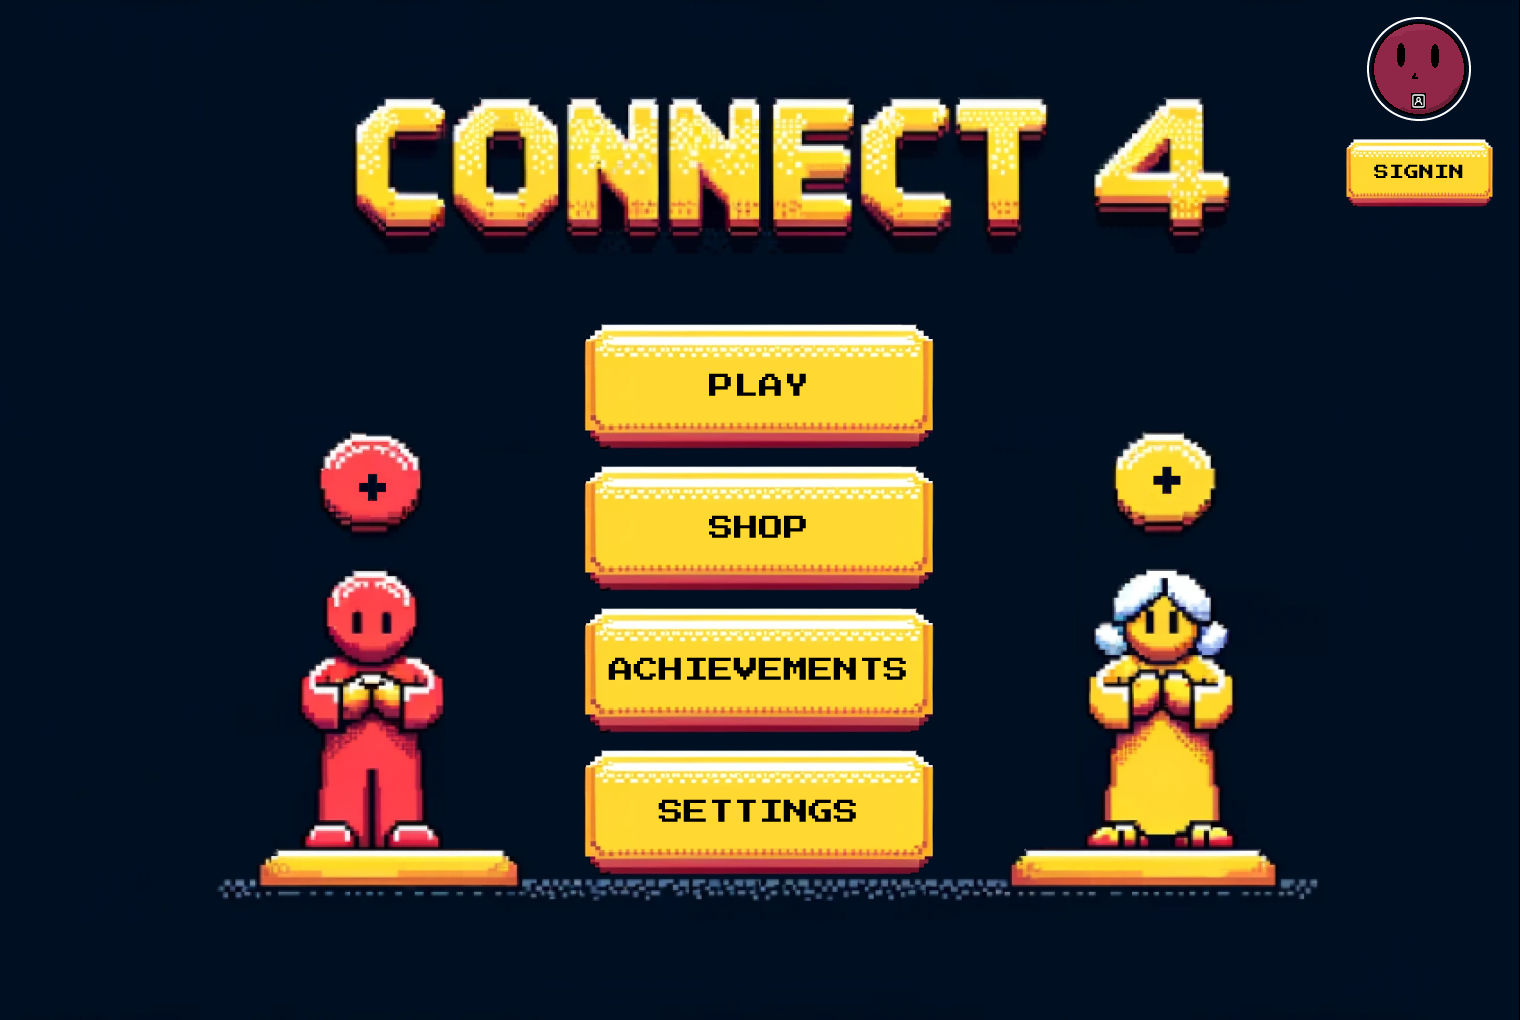
\includegraphics[width=0.8\textwidth]{Menu.png}
  \caption{ Menu hry.}
  \label{fig:menu_label}
\end{figure}

\subsection*{Hracia plocha:}
\begin{figure}[H]
  \centering
  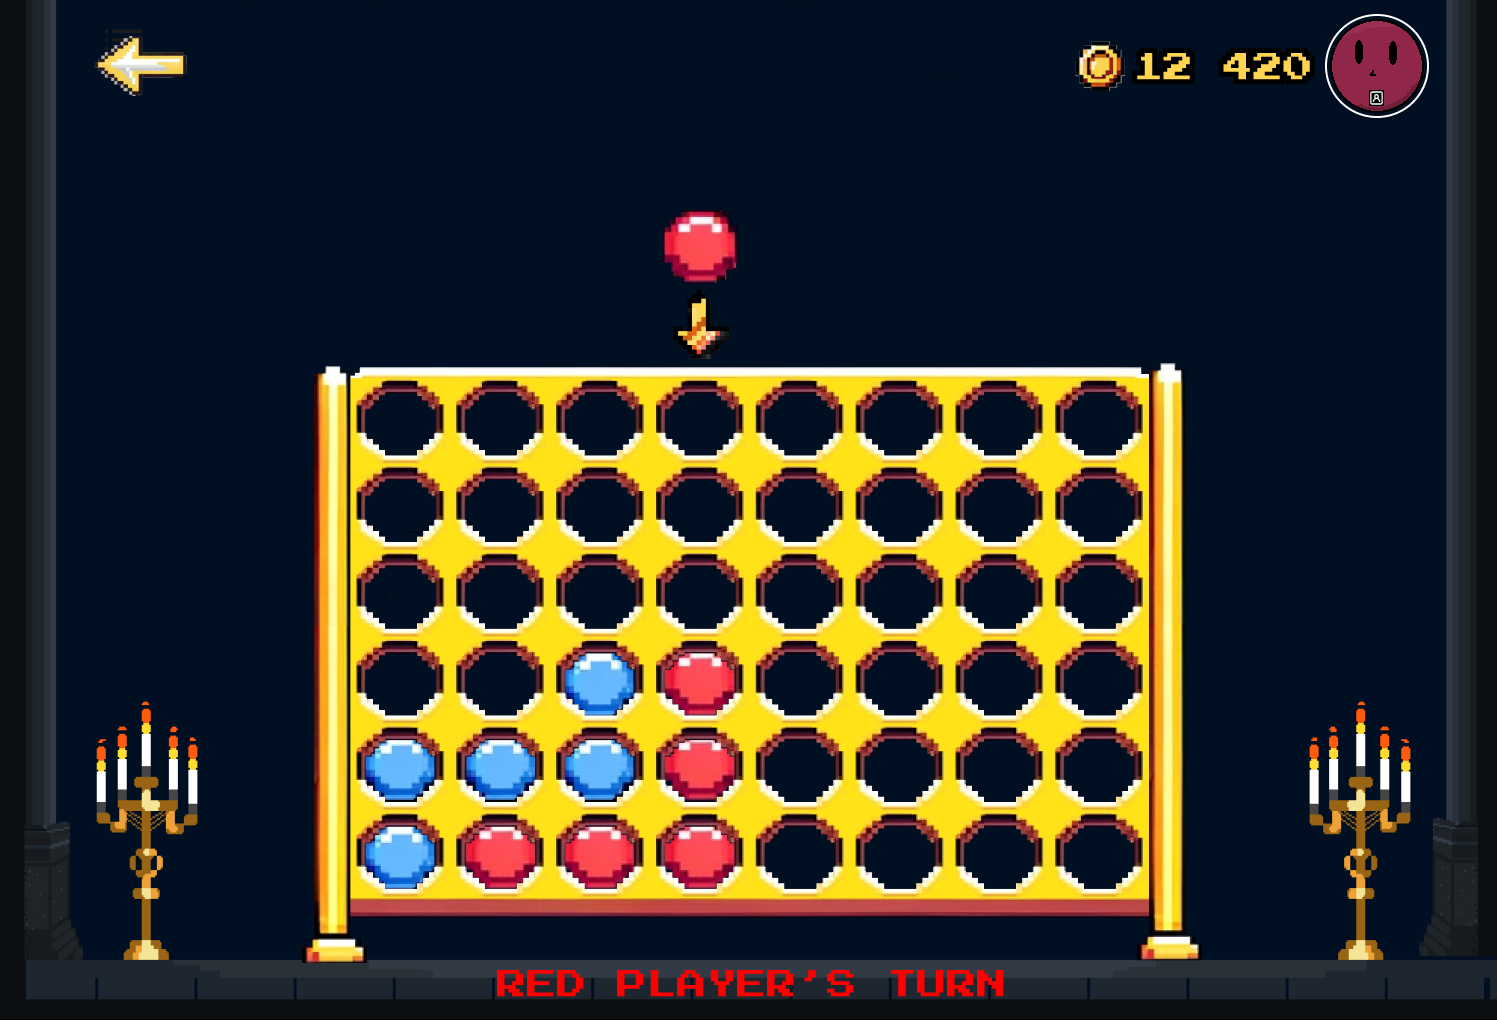
\includegraphics[width=0.8\textwidth]{Plocha.png}
  \caption{ Hracia plocha pre štandardnú verziu.}
  \label{fig:štandard_label}
\end{figure}

\subsection*{Modálne okno sumarizácie hry:}
\begin{figure}[H]
  \centering
  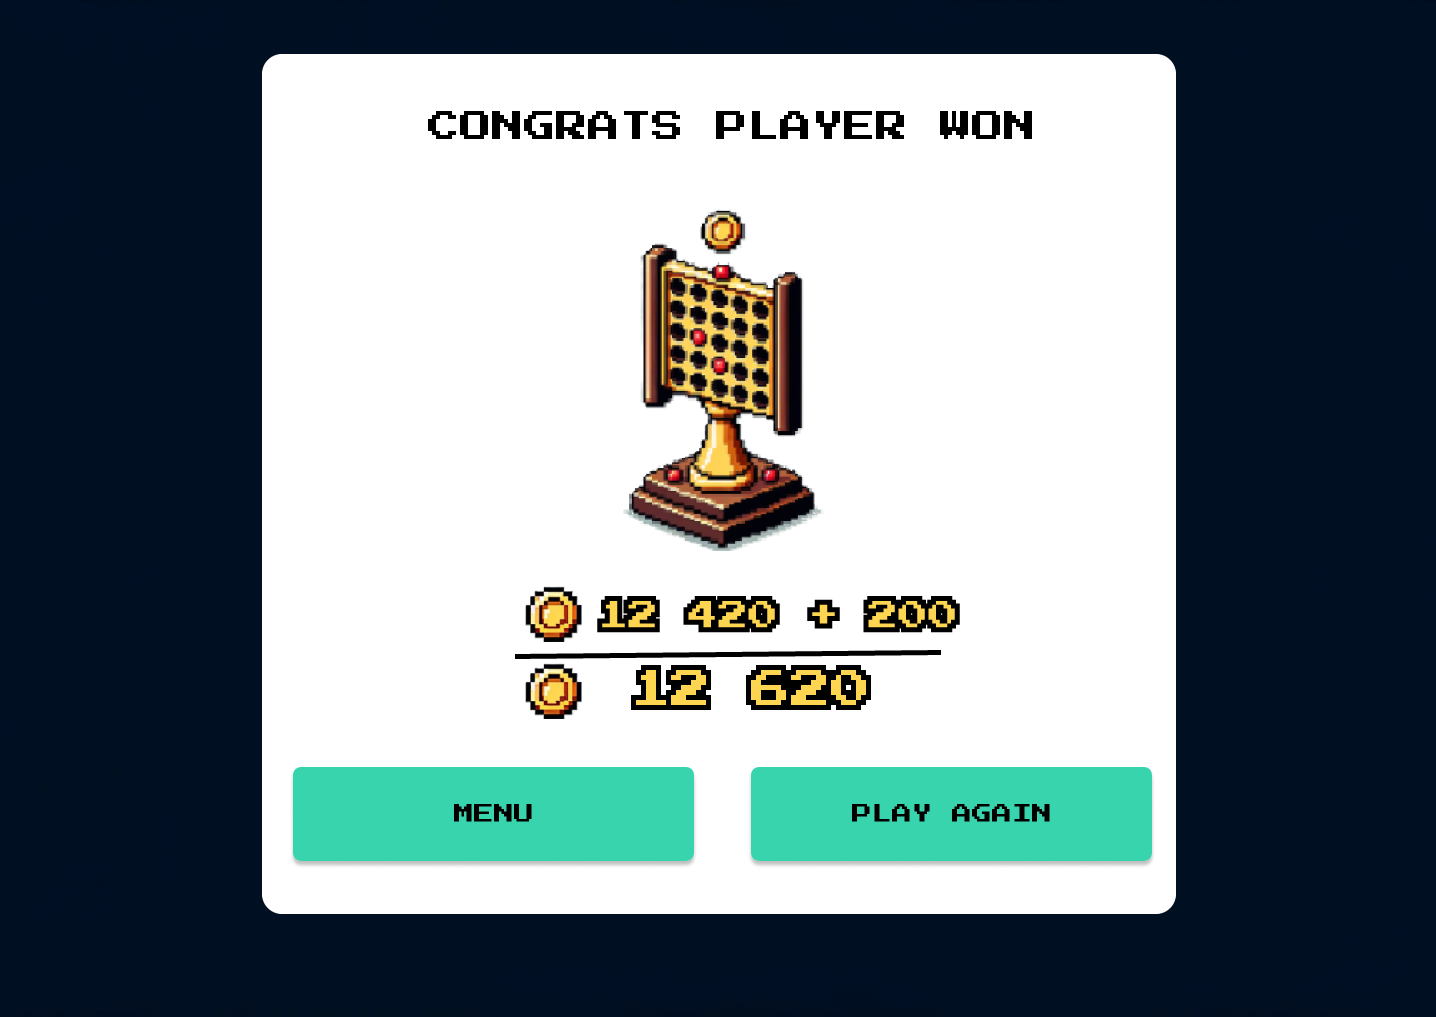
\includegraphics[width=0.8\textwidth]{Vyhra.png}
  \caption{ Sumár po odohraní partie.}
  \label{fig:sumár_label}
\end{figure}
\subsection*{Riešenie potrieb užívateľov}
\begin{enumerate}
  \item \textbf{Zlepšenie užívateľského rozhrania:} Makety znázorňujú, že sme aktualizovali užívateľské rozhranie hry "Connect 4" s cieľom zvýšiť jeho intuitívnosť a vizuálnu atraktivitu. Rozloženie menu a možnosti sú jasne definované a prístupné.
  \item \textbf{Zlepšenie grafiky a vizuálnych efektov:} Namiesto nudných a už zaužívaných prvkou sme sa rozhodli pre viacej atraktívnejšiu formu uživaťeľského prostredia ktorou je "pixelart". Táto voľba nám dovolila si vo vlastnej réžií navrhnúť a nakresliť väčšinu prvkov čo vyustilo k estetickému dizajnu.
  \item \textbf{Možnosť hrať s priateľmi:} Hra je navrhnutá tak aby vedeli dvaja hráči hrať na jednom zariadení a intuitívne zistili v akom štádiu hra je a čo robiť.
\end{enumerate}

\subsection*{Testovanie makety}
\textbf{Testovacia úloha/scenár:} 
\begin{itemize}
  \item Zahrať štandardnú hru a potom navigovať naspäť do menu alebo zahrať daľšiu a potom následovať do menu.
  \item Nájasť cestu k registrácií uživaťeľa a naspäť do menu.
  \item Zorientovať sa v  každom okne a verbálne mi povedať ktoré prvky k čomu slúžia.
\end{itemize}

\textbf{Metriky:}
\begin{itemize}
    \item \textbf{Úspešnosť dokončenia scenára/úlohy (success/error rate):} Koľko používateľov bolo schopných úspešne dokončiť úlohu?
    \item \textbf{Počet pokusov o nájdenie informácie (number of trials):} Koľkokrát používateľ klikol alebo navštívil rôzne časti rozhrania, kým našiel správnu informáciu?
    \item \textbf{Počet dotazov od používateľa:} Koľkokrát používateľ požiadal o pomoc alebo mal dotaz týkajúci sa postupu?
    \item \textbf{Úspešnosť nájdenia predpokladanej cesty pri navigácii (expected path):} Sledujte, či používateľ nasledoval predpokladanú cestu k dosiahnutiu cieľa.
\end{itemize}

\textbf{Respondenti:}

Počet: 3 

Poznámka: Rovnakí ako pri dotazníku.

\subsection*{Vyhodnotenie metrík:}
\begin{itemize}
    \item \textbf{Úspešnosť dokončenia scenára/úlohy (success/error rate):} 66\%
    \item \textbf{Počet pokusov o nájdenie informácie (number of trials):} V priemere 2.
    \item \textbf{Počet dotazov od používateľa:} V priemere 1.
    \item \textbf{Úspešnosť nájdenia predpokladanej cesty pri navigácii (expected path):} 100\%
\end{itemize}

\subsection*{Vyhodnotenie:}
Test odhalil nedostatok pri navigácií do rozhrania registrácie nového uživaťeľa. V aktuálnej verzí sa k tejto obrazovke dostáva cez obrazovku MENU-LOGIN-REGISTER.
Uživaťeľovi to nakoniec došlo no trvalo mu to dlhšie než by som očakával (úloha 2.). Ako riešenie plánujem pridať tlačítko pre registráciu priamo do Menu aplikácie.
Ďaľšia maličkosť nastala pri jednom respondentovi kedy po kliknutí na tlačidlo play sa zamyslel ktorý herný režim vybrať.
A spýtal sa čo znamená crazy house. Pre opravenie tohoto problému plánujem pridať vysvetlivky ktoré sa  zobrazia po nájdení myšou na konkrétnu hernú možnosť.
Čo neodhalili ani respondenti ale prišiel som na to pri ich pozorovaní.Keď je niekto prihlásený, berieme túto osobu za hlavného užívateľa. Preto vzniká otázka,
či by sme mali zobrazovať výhru druhého hráča alebo prehru prvého hráča.
Riešenie tohoto problému by malo byť zobrazenie  len výhry kedže obaja sedia za spoločným zariadením.
Kedže som použil tých istých respondentov ako v dotazníku mohol som sa spýtať či si aplikáciu predstavovali takto.
Odpovede boli kladné. Najviac si pochvaľovali zaujímavý dizajn a možnosť rýchlej hry bez registrácie.

\subsection{(Majer)}
\subsection*{Vytvorenie konta}
\begin{figure}[H]
  \centering
  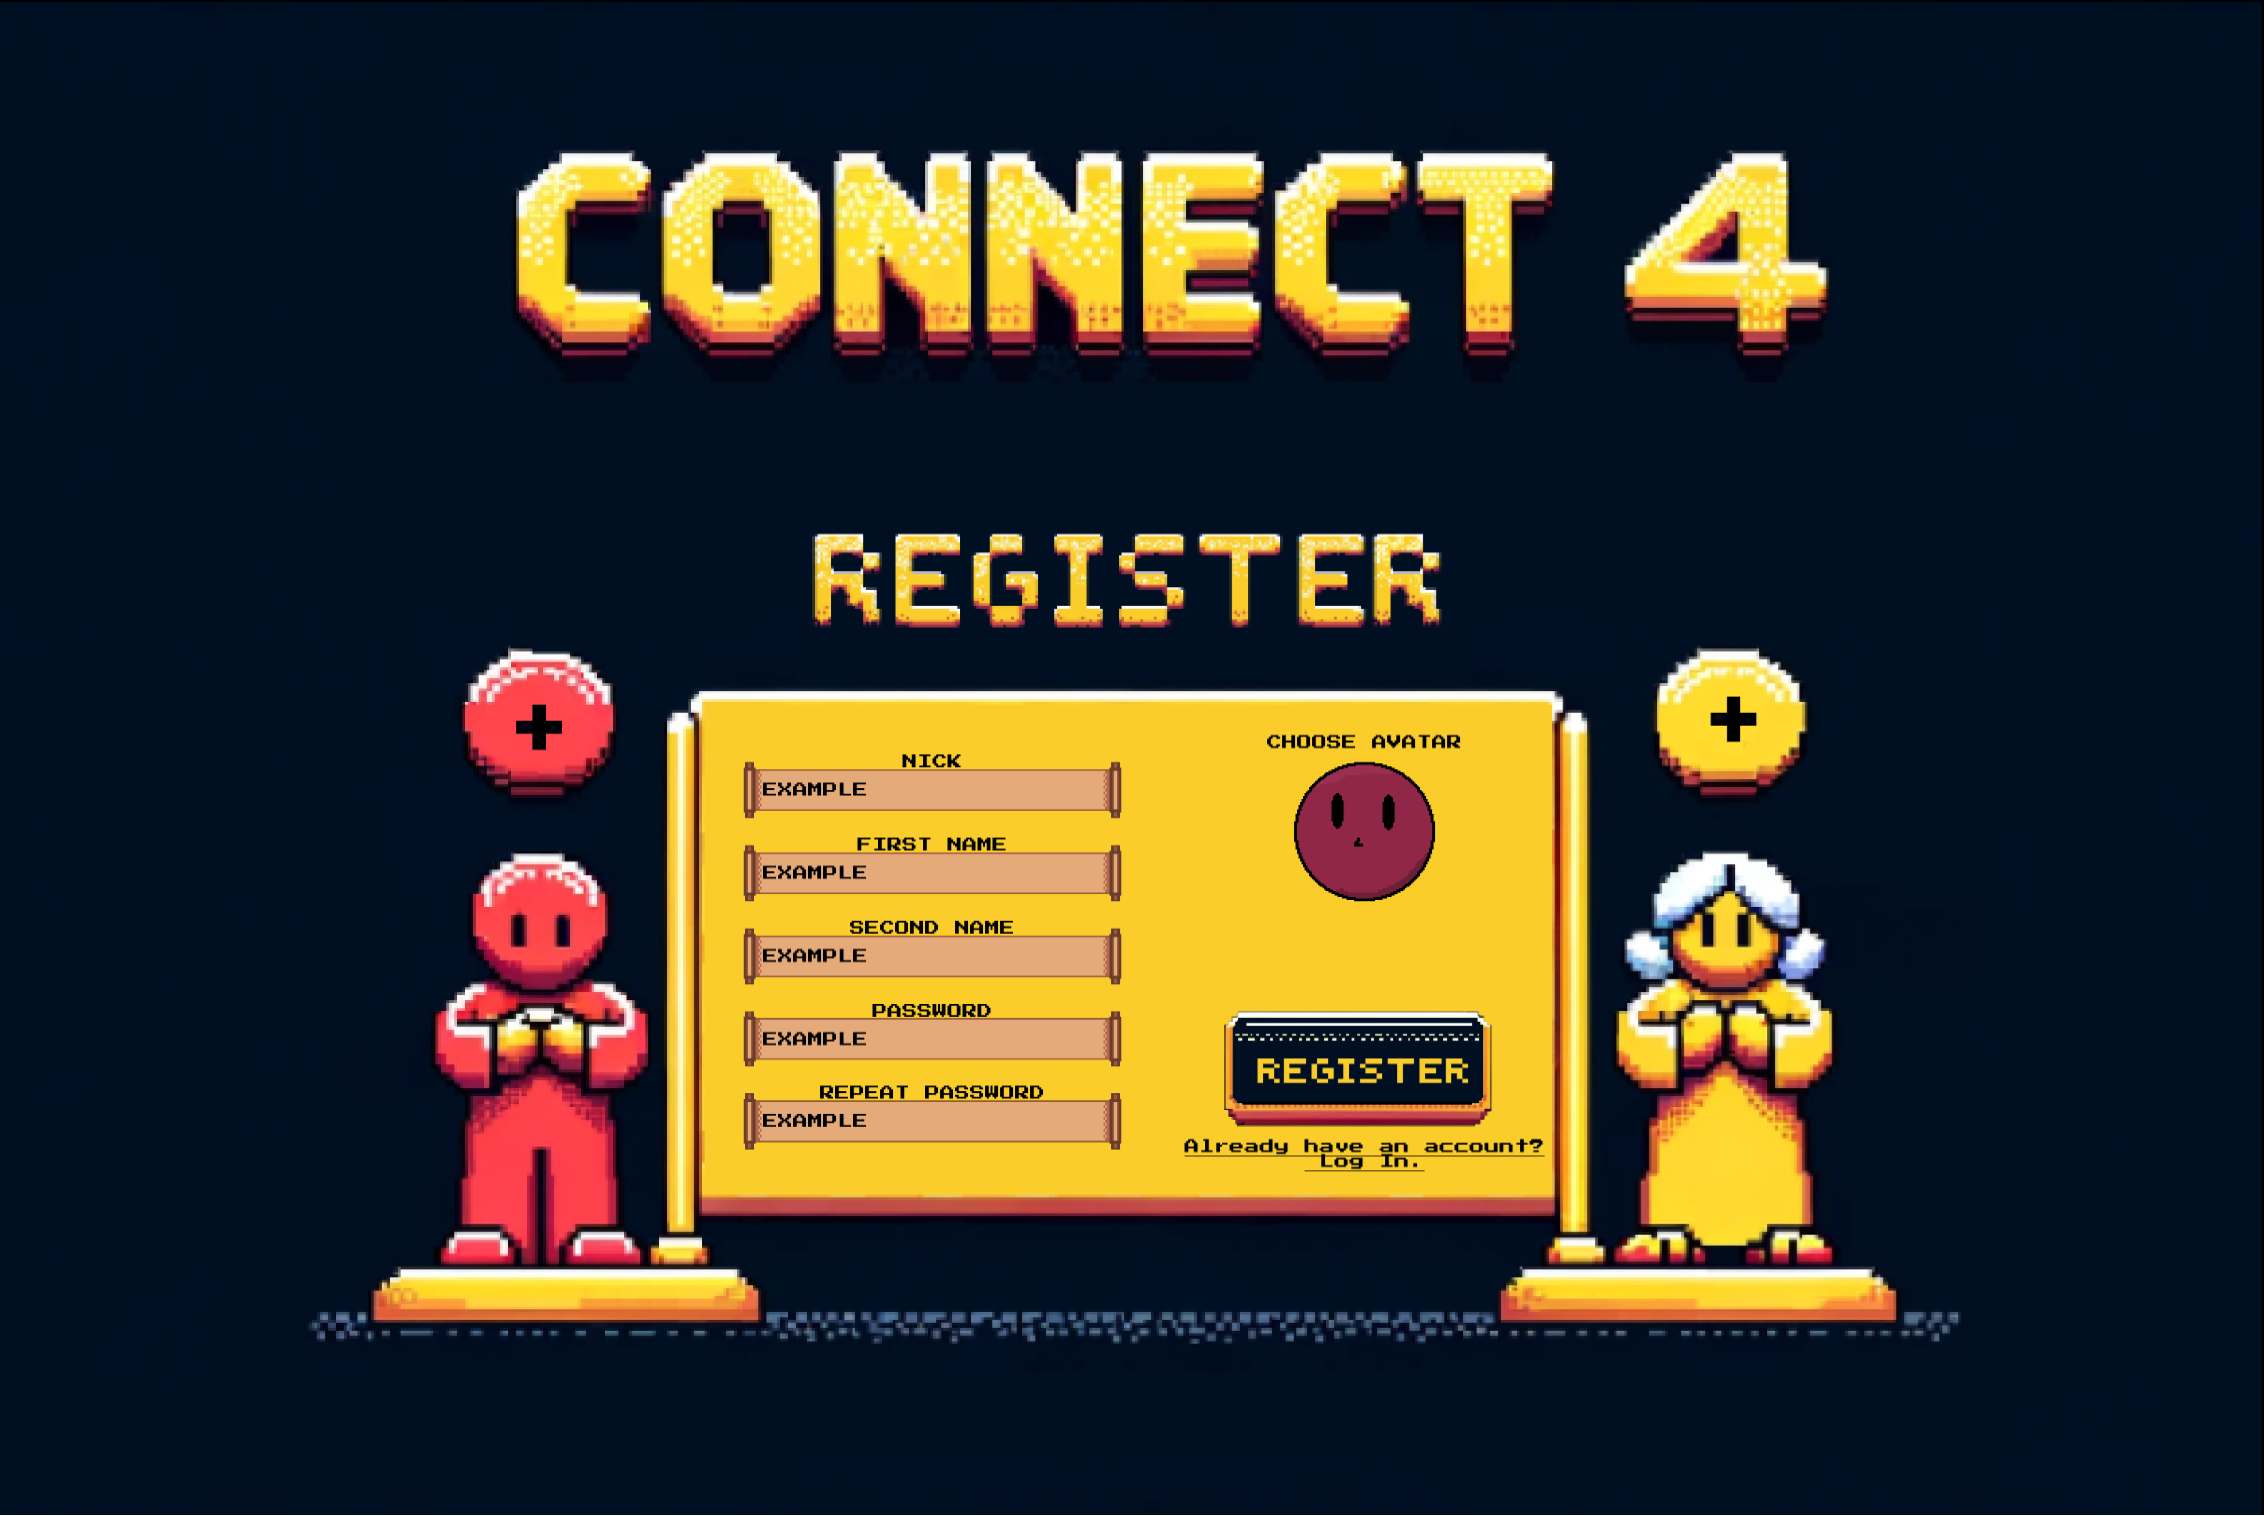
\includegraphics[width=0.8\textwidth]{Register.png}
  \caption{Vytvorenie nového konta}
  \label{fig:register}
\end{figure}

\subsection*{Úspešné vytvorenie konta}
\begin{figure}[H]
  \centering
  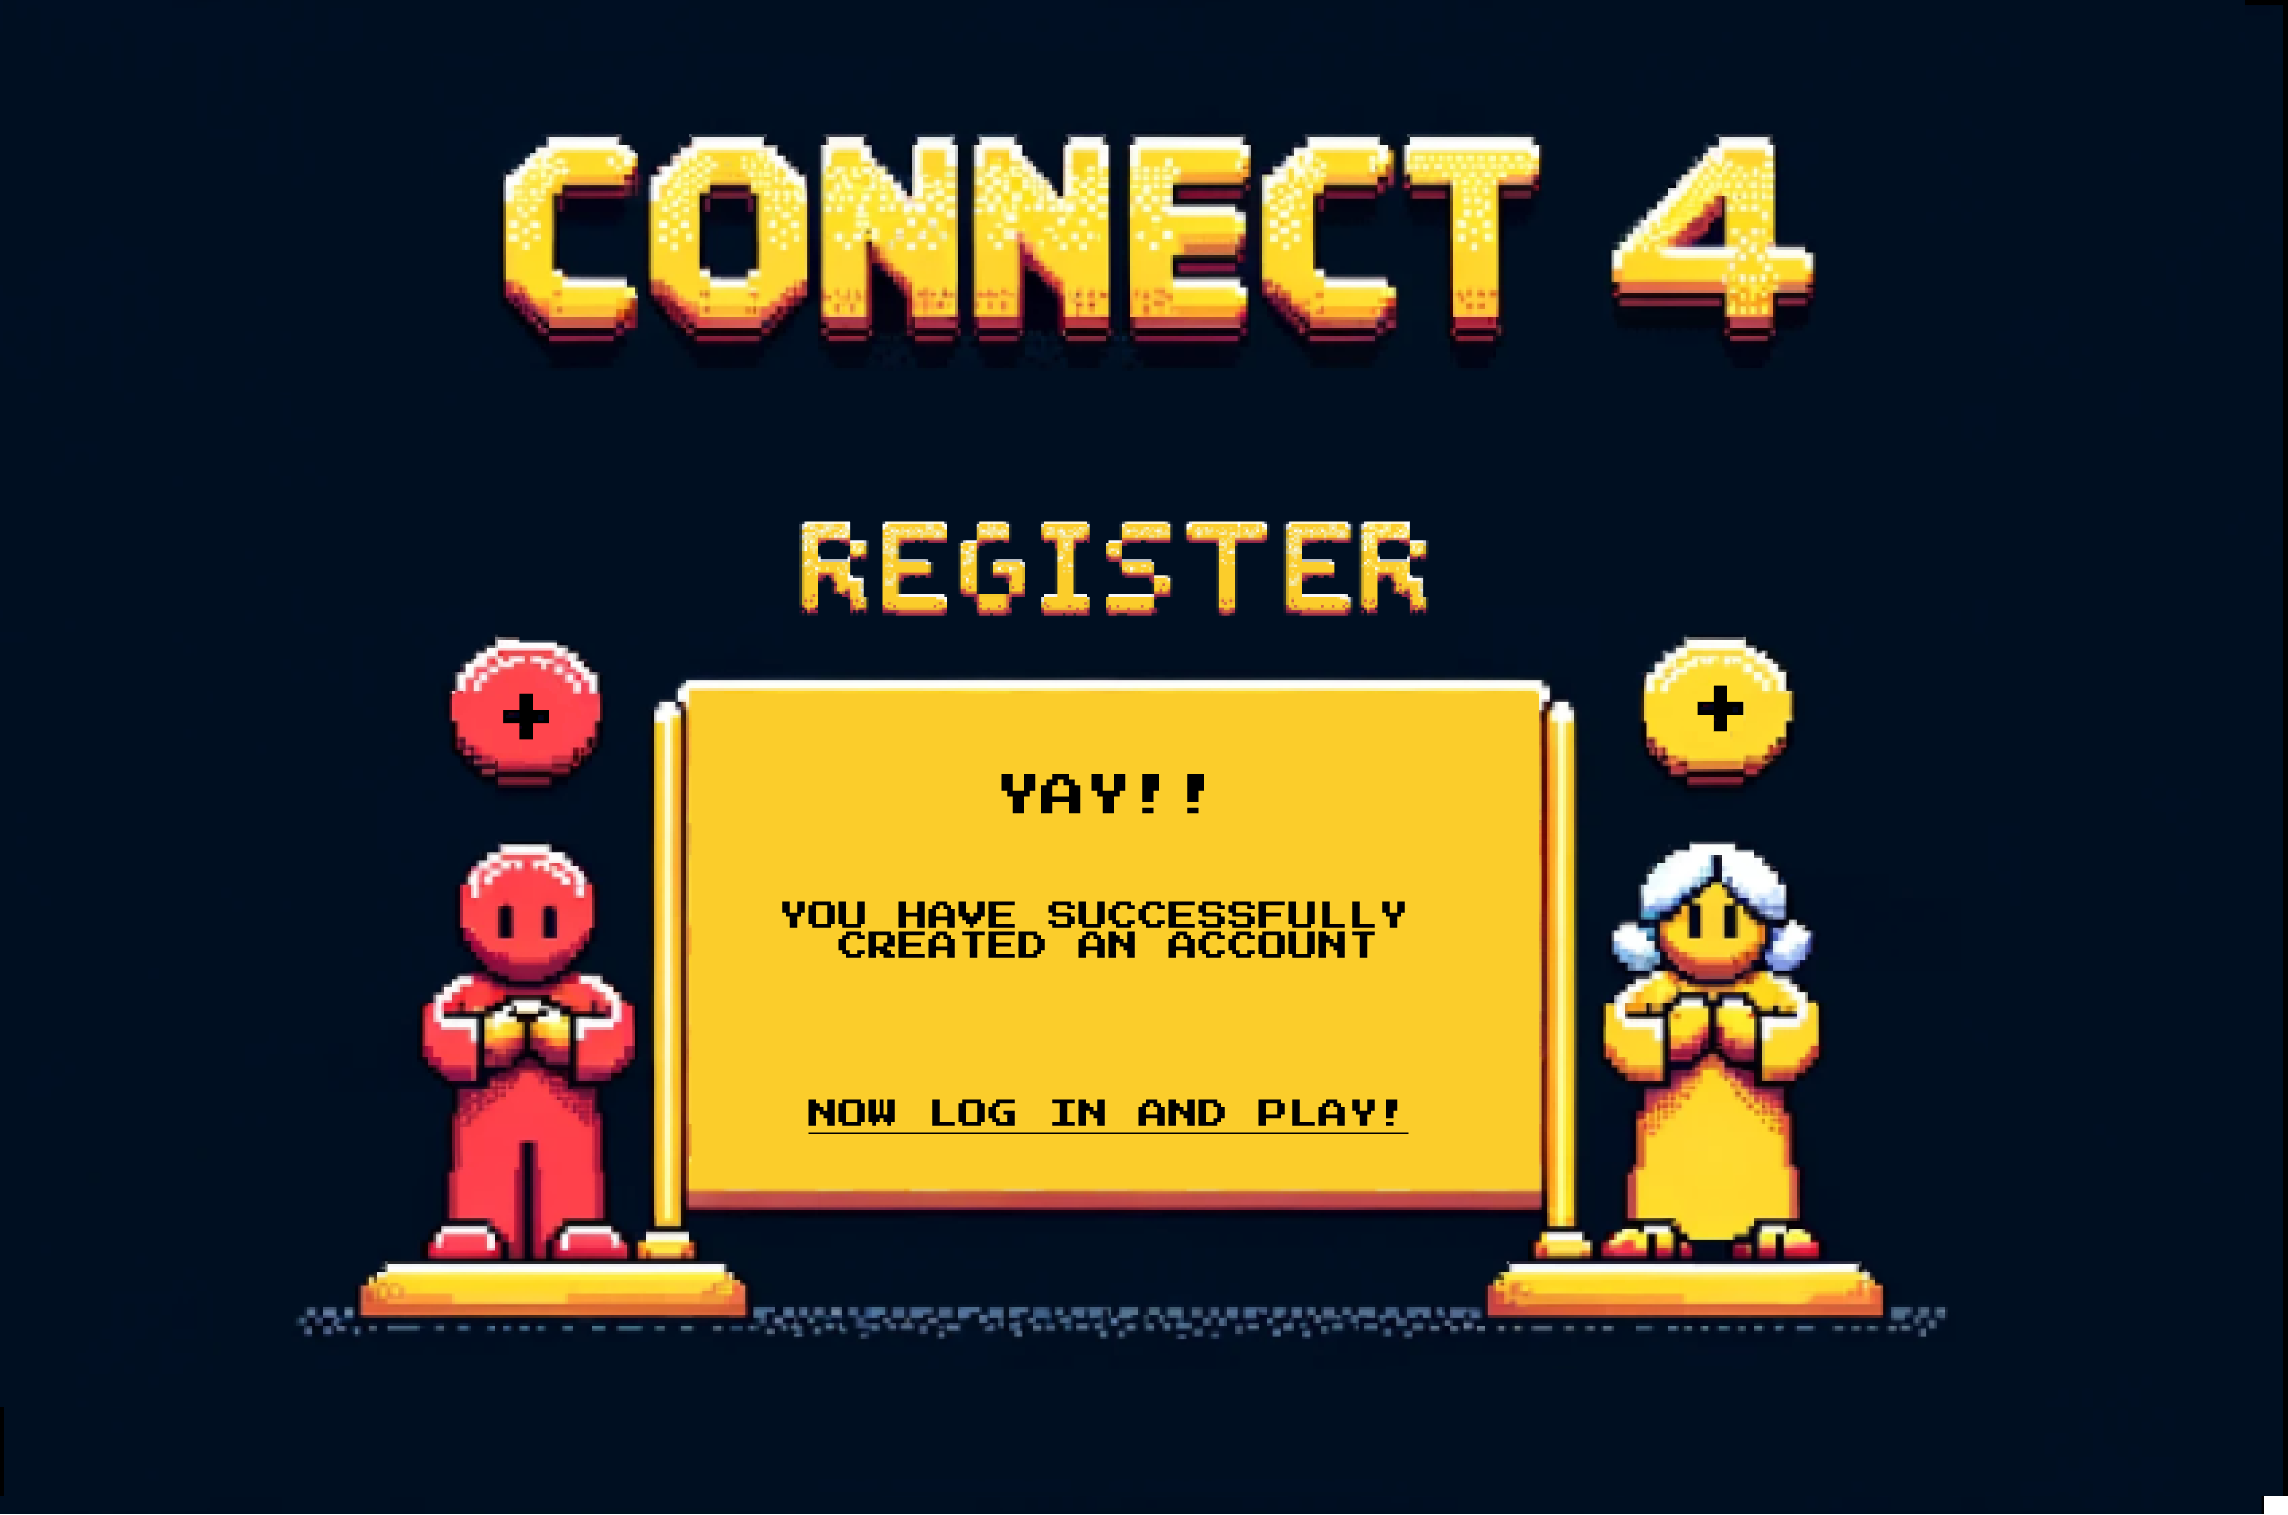
\includegraphics[width=0.8\textwidth]{RegisterDone.png}
  \caption{Úspešné vytvorenie konta}
  \label{fig:register_done}
\end{figure}

\subsection*{Prihlásenie sa}
\begin{figure}[H]
  \centering
  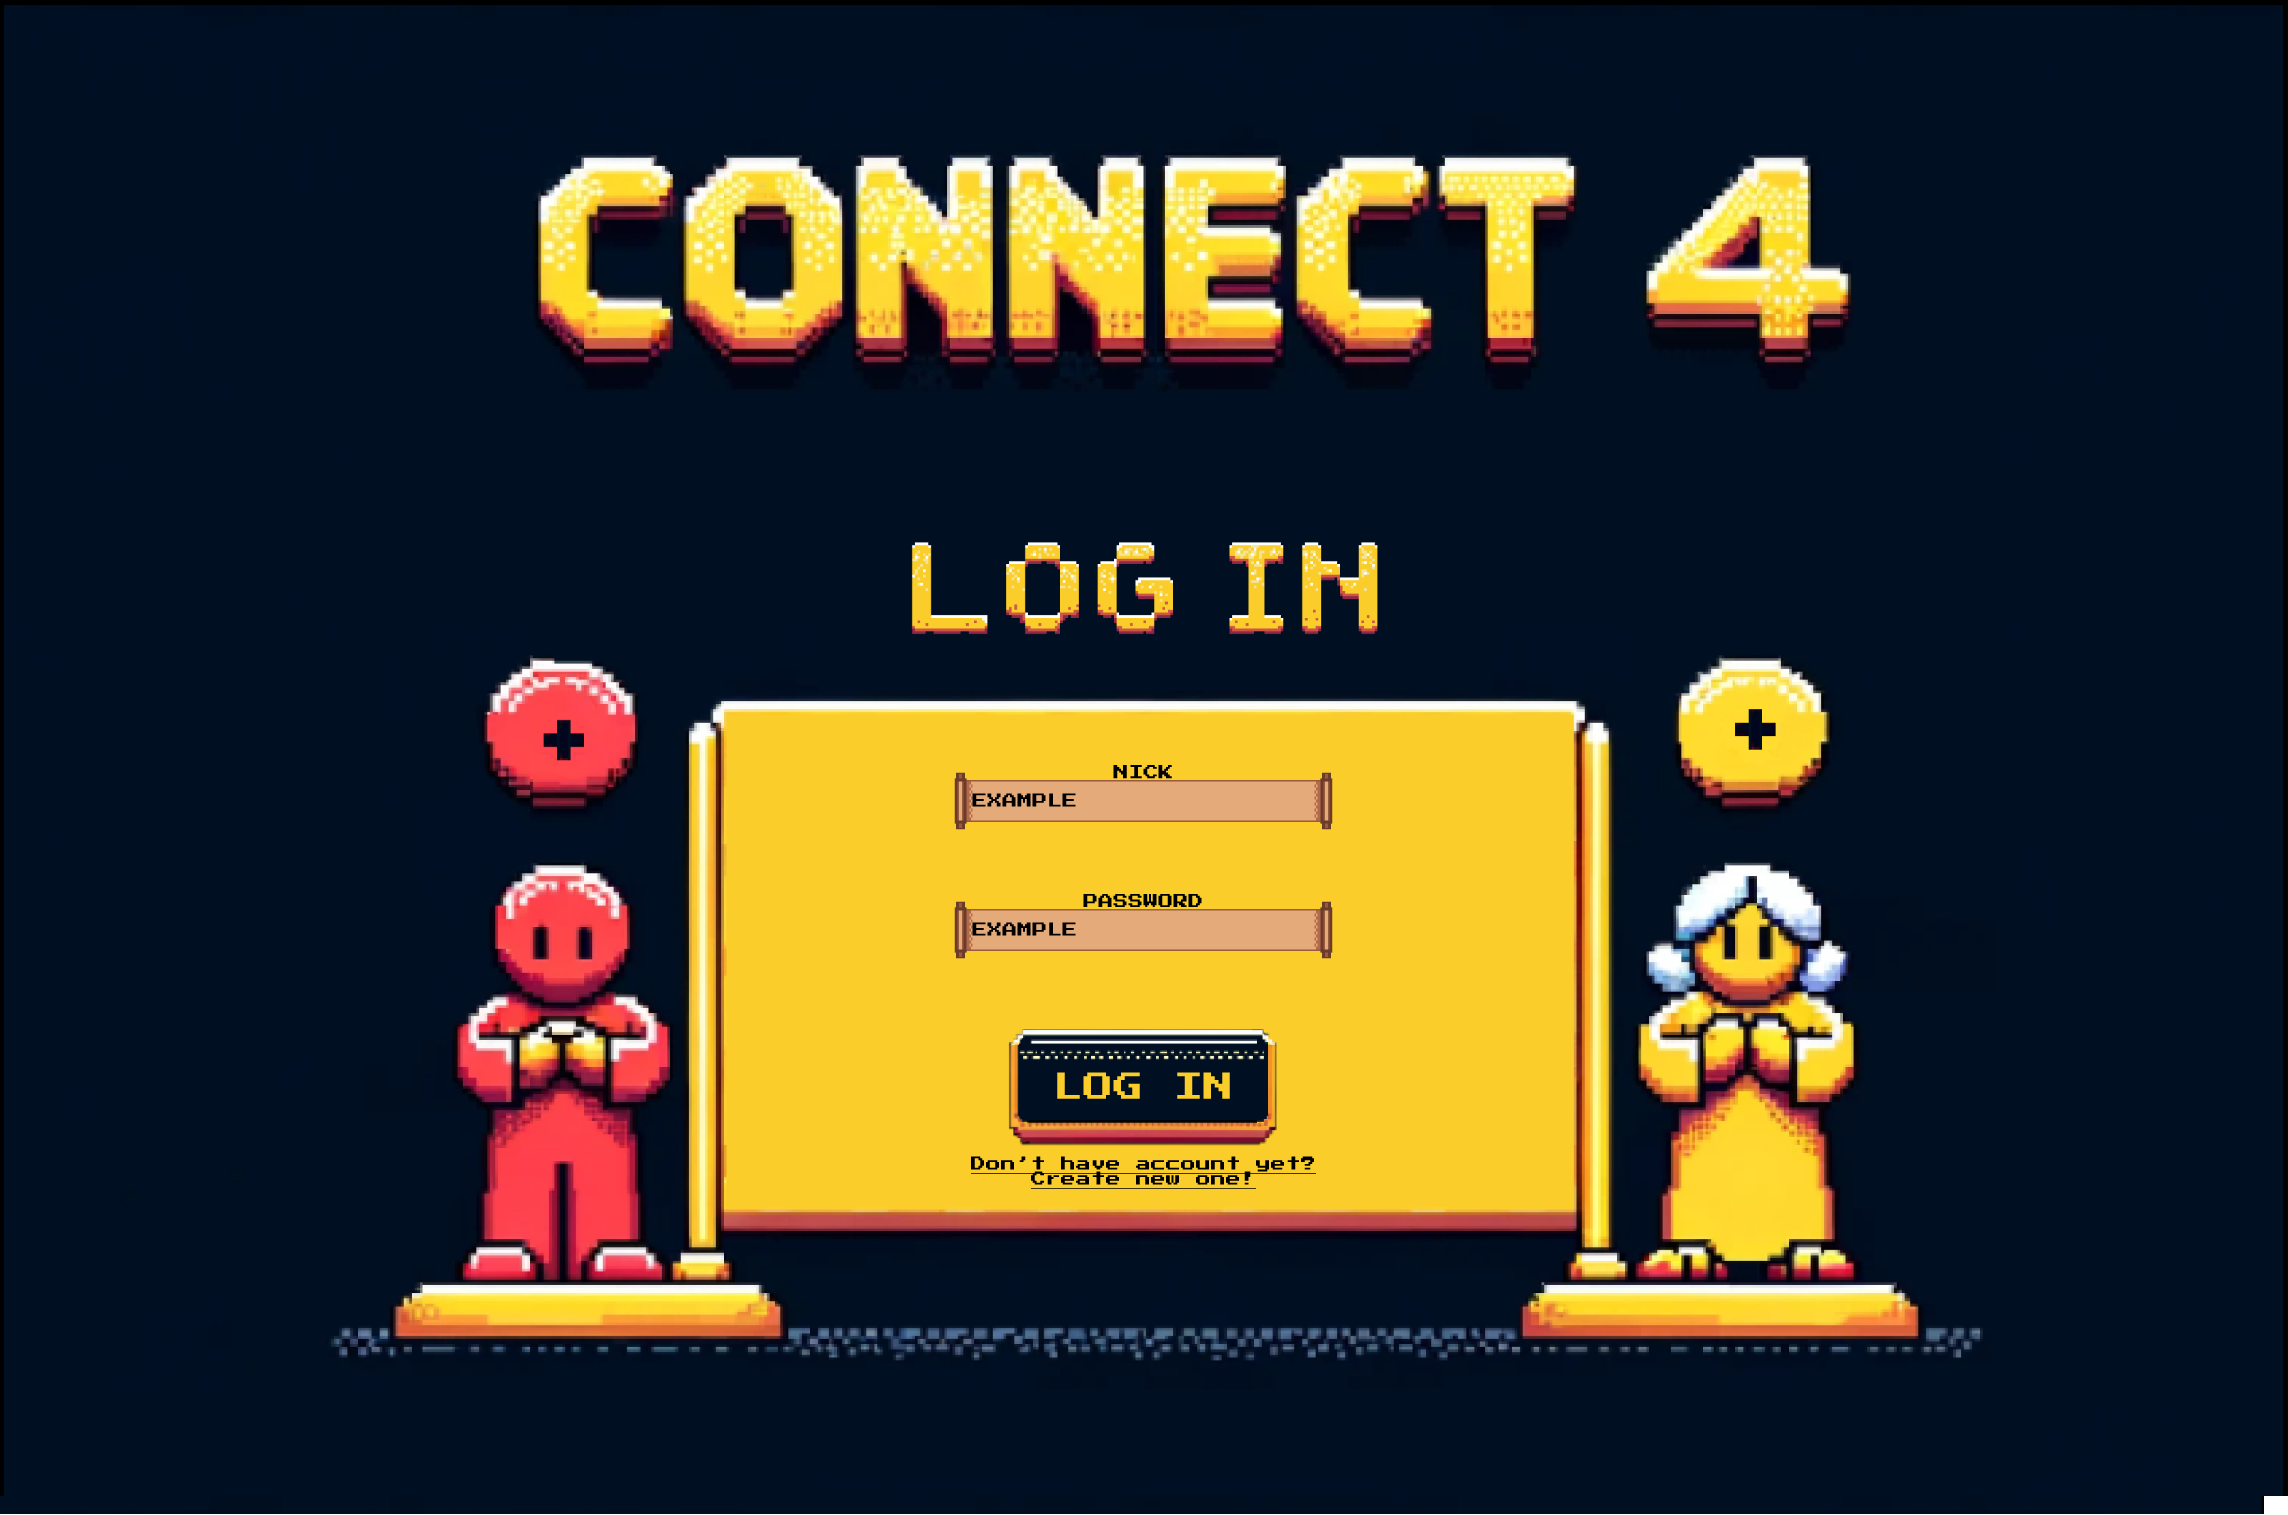
\includegraphics[width=0.8\textwidth]{LogIn.png}
  \caption{Prihlásenie sa do existujúceho konta}
  \label{fig:login}
\end{figure}

\subsection*{Výber hernej varianty}
\begin{figure}[H]
  \centering
  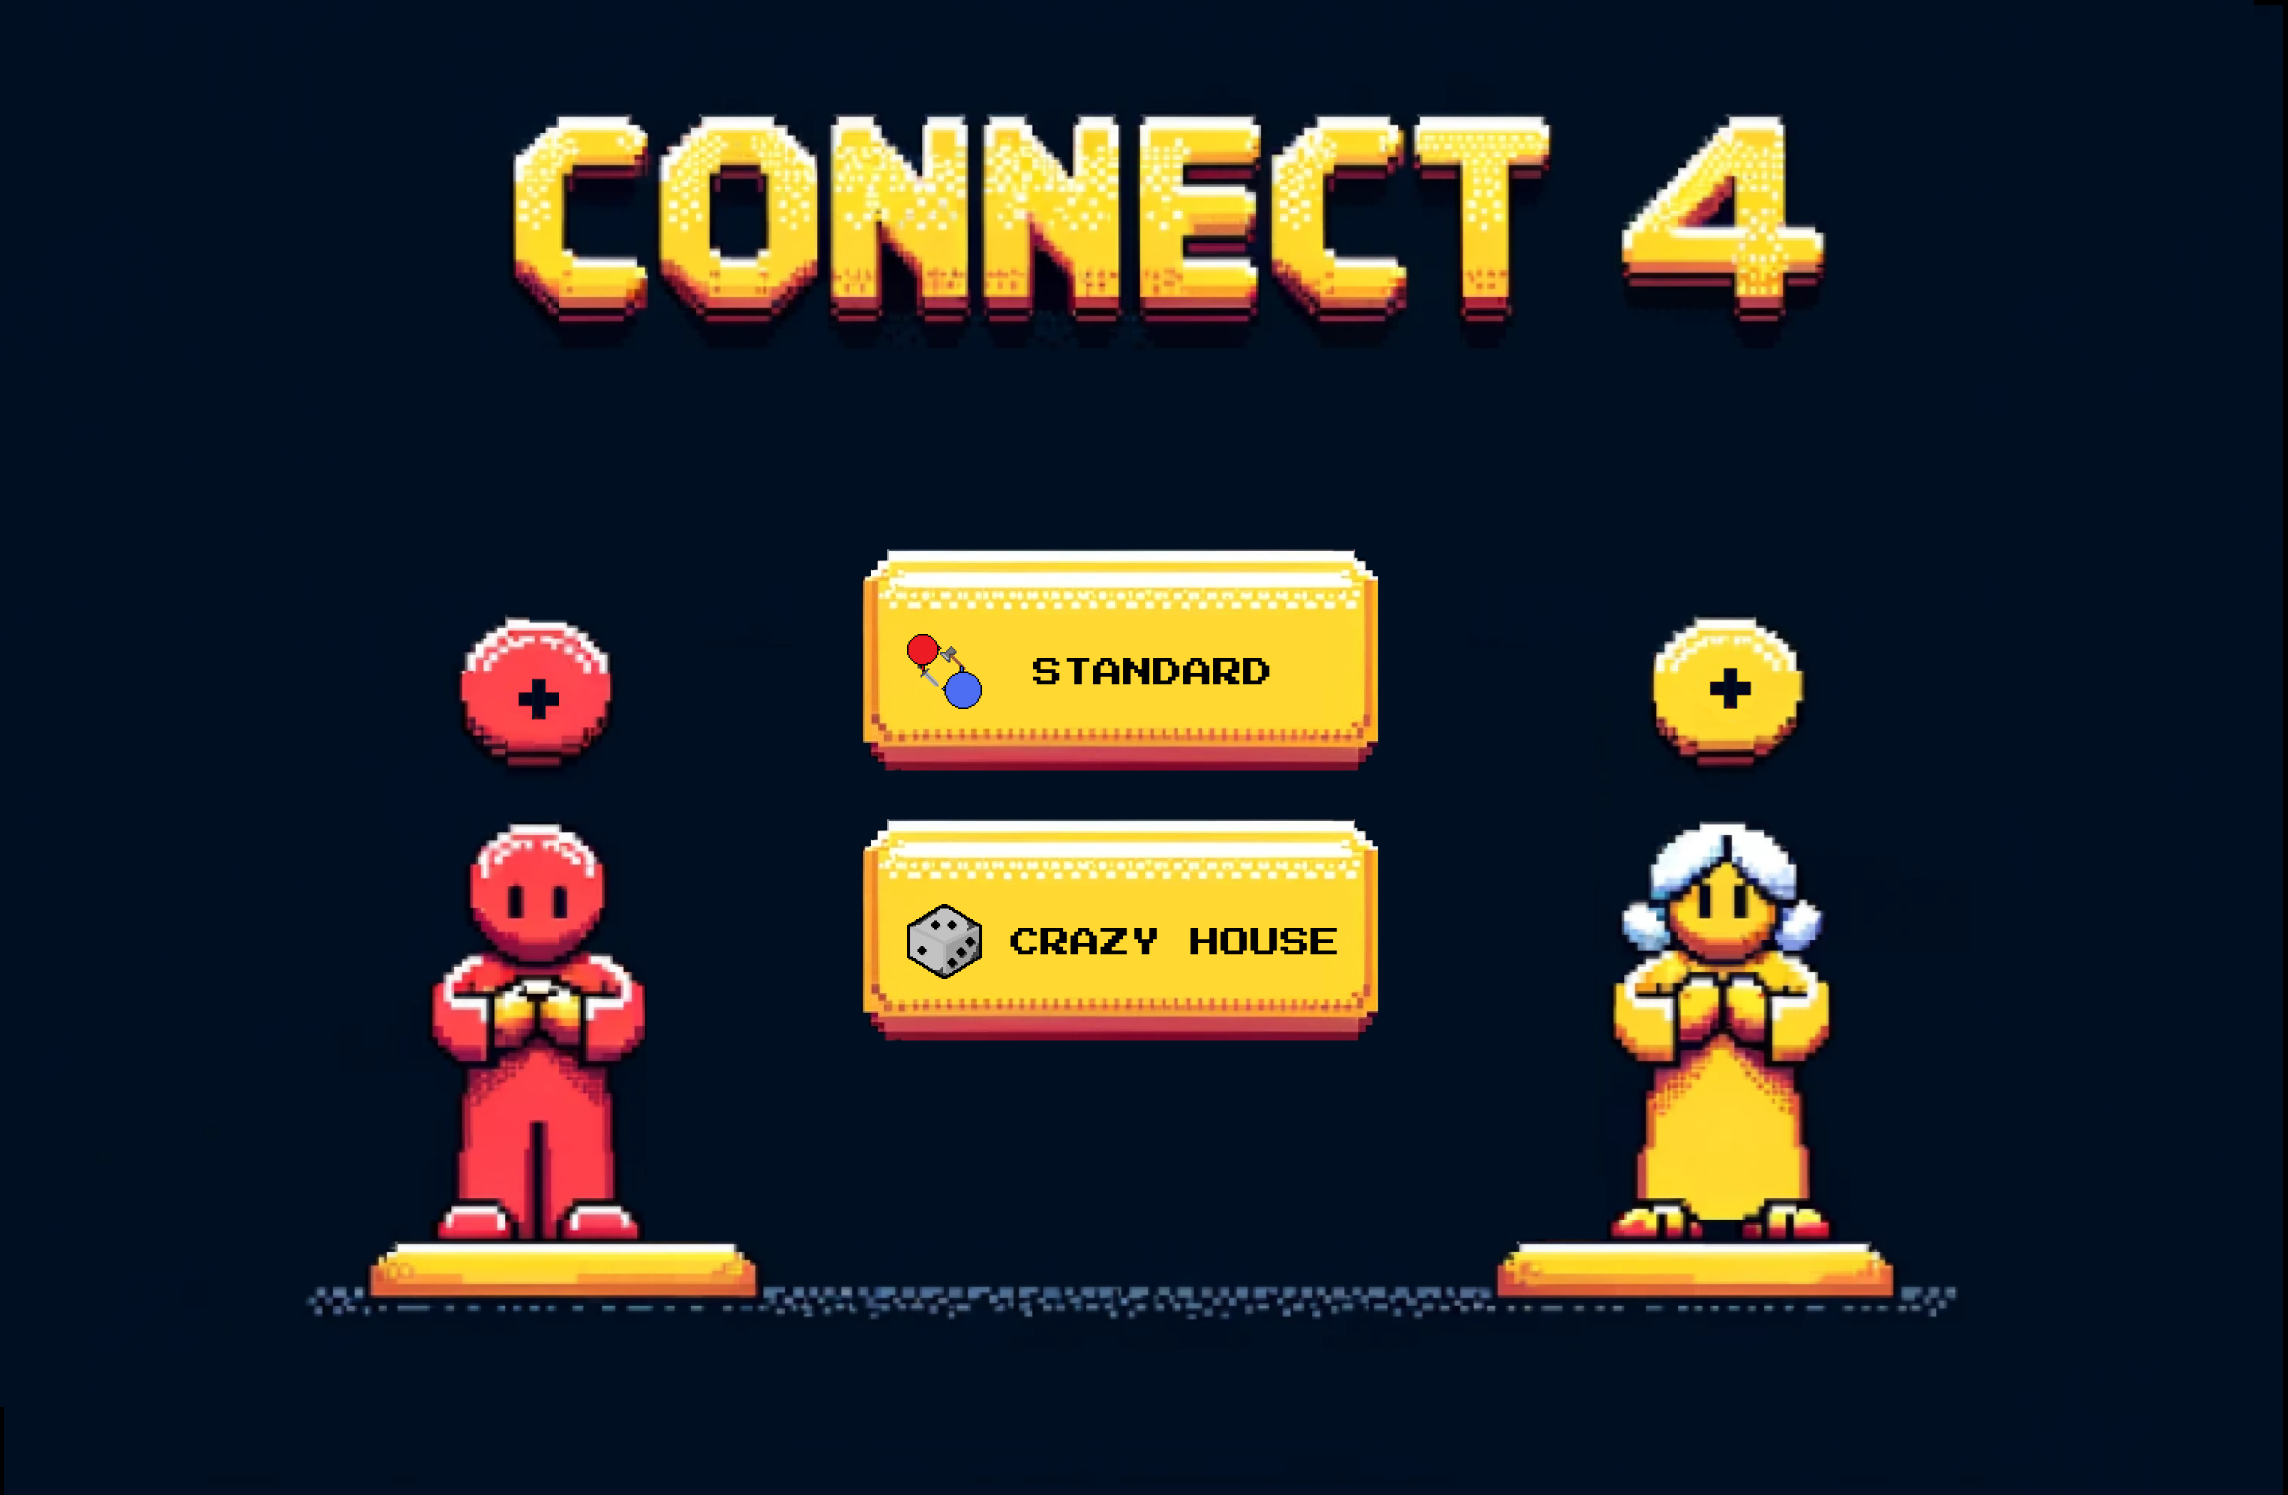
\includegraphics[width=0.8\textwidth]{PickVariant.png}
  \caption{Výber varianty hry štyri v rade}
  \label{fig:pick_variant}
\end{figure}

\subsection*{Varianta hry s náhodnosťou}
\begin{figure}[H]
  \centering
  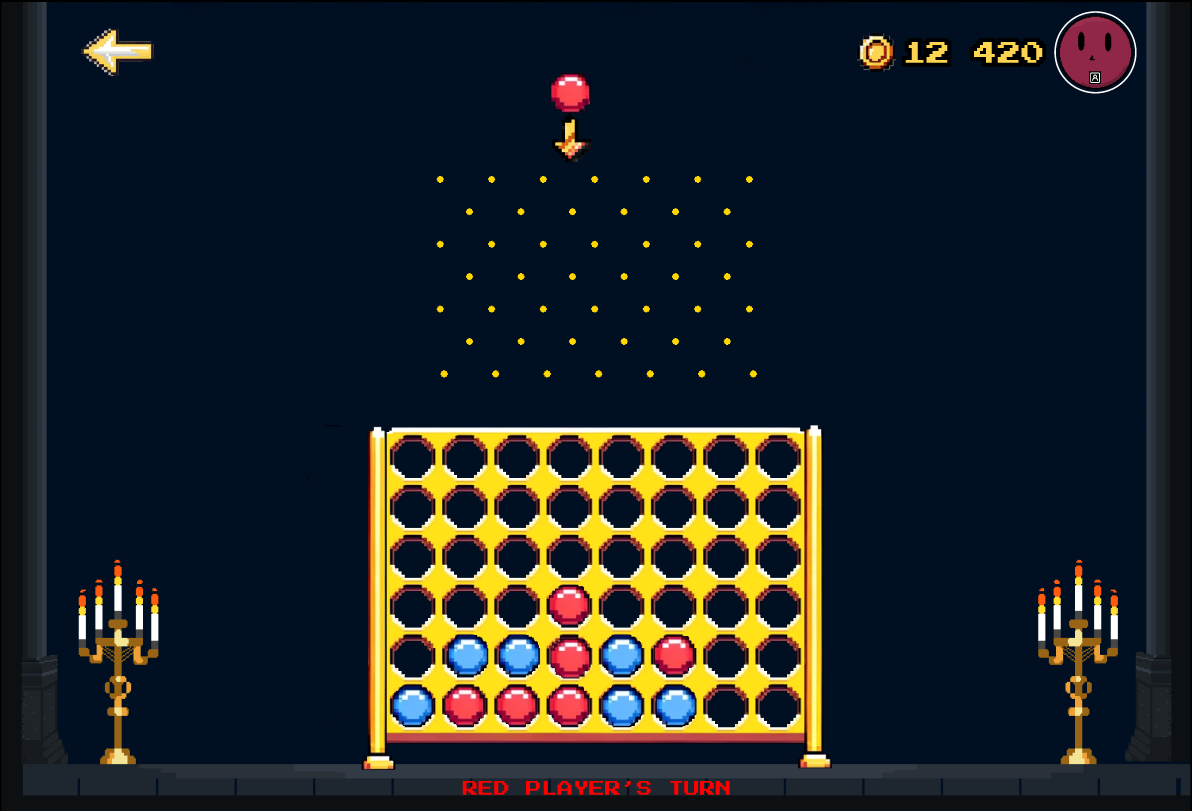
\includegraphics[width=0.8\textwidth]{RandomVariant.png}
  \caption{Varianta hry štyri v rade s náhodnosťou}
  \label{fig:random_variant}
\end{figure}

\subsection*{Riešenie potrieb užívateľov}
\begin{itemize}
  \item \textbf{Modifikovateľnosť:} Pokiaľ sa užívateľ prihlási, má možnosť zmeny 
               použitej scenérie na pozadí hry, avataru profilu a tokenu použitého pri hre.
  \item \textbf{Varianty:} Pridali sme variantu hry, ktorá má za úlohu udržať hru čo najdlhšie
                zaujímavú. Ide o variantu kde pri páde tokenu do hernej plochy, sa token
                ešte môže poodrážať a dopadnúť na iné políčko ako bolo pôvodne zamýšlané.
  \item \textbf{Vizuálny aspekt:} Rozhodli sme sa využiť pixel art ako zvolenú umeleckú formu.
                Zámienkou je vytvoriť atraktívnu hru pre nových užívateľov ako aj pre stálich hráčov.
\end{itemize}

\subsection*{Testovanie Makety}
Pri testovaní makety boli oslovení tí istí štyria hráčí hry štyri v rade ako pri
vyplňovaní dotazníku. Pre testovanie boli vytvorené scenáre, ktorými mali 
subjekty prejsť. Testovanie prebiehalo cez videohovor, takže boli sledované všetky
dotazy a návrhy na zlepšenie. Ako metriku som použil úspešnosť dokončenia úlohy a
počet dotazov.\\
Nižšie sú uvedené scenáre pripravené pre testované subjekty:
\begin{itemize}
  \item Dostať sa z menu do registrácie, vytvoriť si konto a prihlásiť sa
  \item Dostať sa z menu do prihlásenia, prihlásiť sa a zapnúť si variantu "Crazy House"
  \item Z varianty hry "Crazy House" sa vrátiť do menu a zapnúť štandardnú hru
\end{itemize}
\subsection*{Vyhodnotenie metrík}
\begin{itemize}
  \item Úspešnosť dokončenia úlohy: 100\%
  \item Počet dotazov: V priemere 2 (niektoré sa opakovali)
\end{itemize}
Všetkým užívateľom sa na prvý pokus podarilo navigovať cez dané scenáre. 
Mali však pár dotazov, ktoré pri ich riešení zjednoduchšia navigáciu v aplikácii a anulujú zmätenie budúcich užívateľov.
Nájdené chyby v aplikácii sú uvedené nižšie:
\begin{itemize}
  \item Jeden zo subjektov poukázal na to že neexistuje možnosť sa dostať z prihlásenia a registrácie naspäť do menu bez toho aby sa prihlásil.
  \item Podobný problém bol nájdený neskôr pri výbere varianty hry, teda chýbaju možnosti návratu do menu.
  \item Jeden zo subjektov, poukázal na to že budúci hráči by mohli byť zmetený z názvu "Crazy House" a teda by tam mali byť pridané vysvetlivky.
\end{itemize}
\subsection*{Riešenie problému}
V aplikácii budú pridané tlačítka pre jednoduchšiu navigáciu medzi stranami.
Pridané budú aj vysvetlivky k variantám hry. ktoré oprostia hráča od pochopenia varianty
štýlom "pokus, omyl".


\subsection{(Mahút)}
\subsection*{Profil}
\begin{figure}[H]
  \centering
  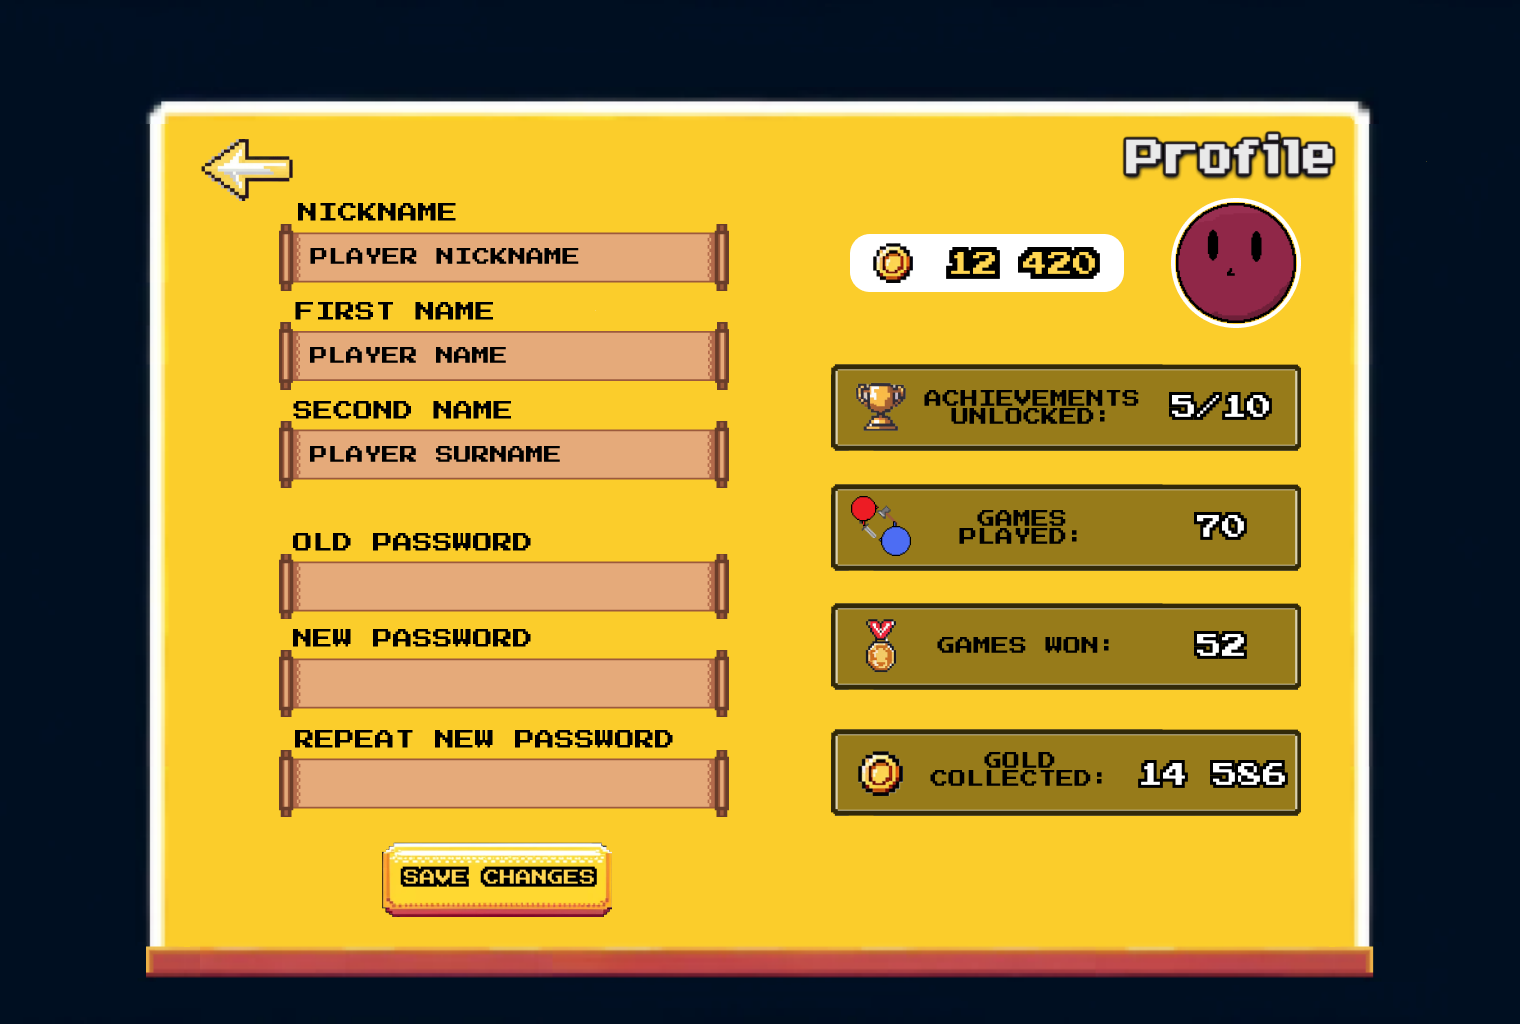
\includegraphics[width=0.8\textwidth]{Profile.png}
  \caption{Stránka profilu so štatistikami}
  \label{fig:profile}
\end{figure}

\subsection*{Úspechy}
\begin{figure}[H]
  \centering
  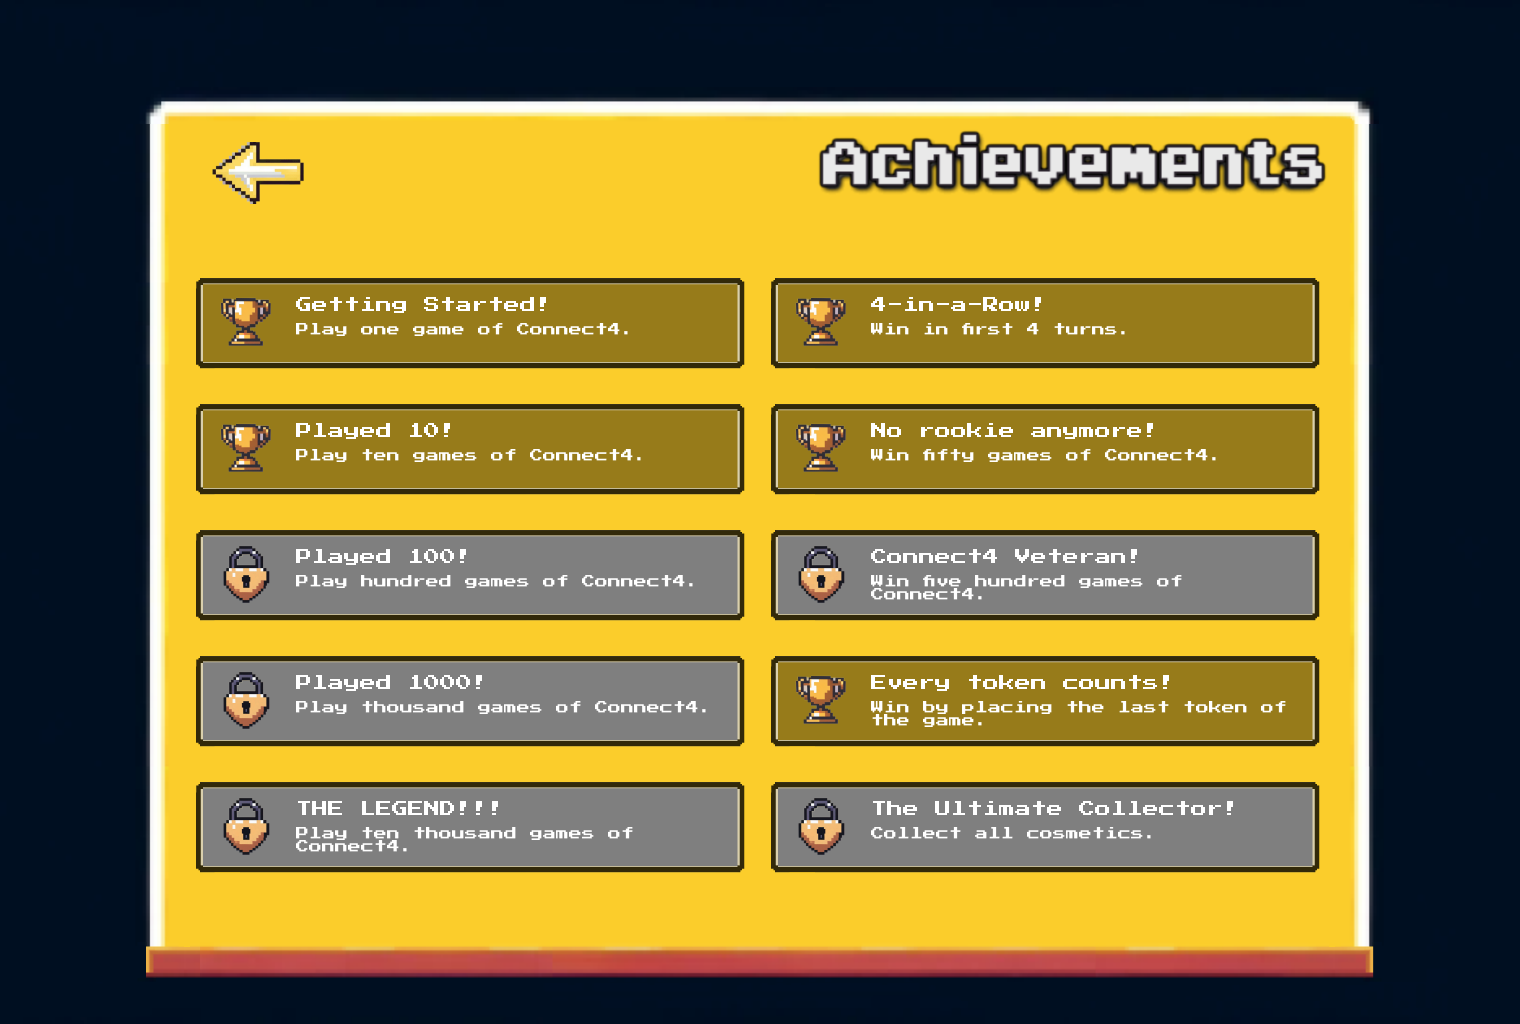
\includegraphics[width=0.8\textwidth]{Achievements.png}
  \caption{Prehľad dosiahnutých a dosiahnuteľných úspechov}
  \label{fig:achievements}
\end{figure}

\subsection*{Nastavenia}
\begin{figure}[H]
  \centering
  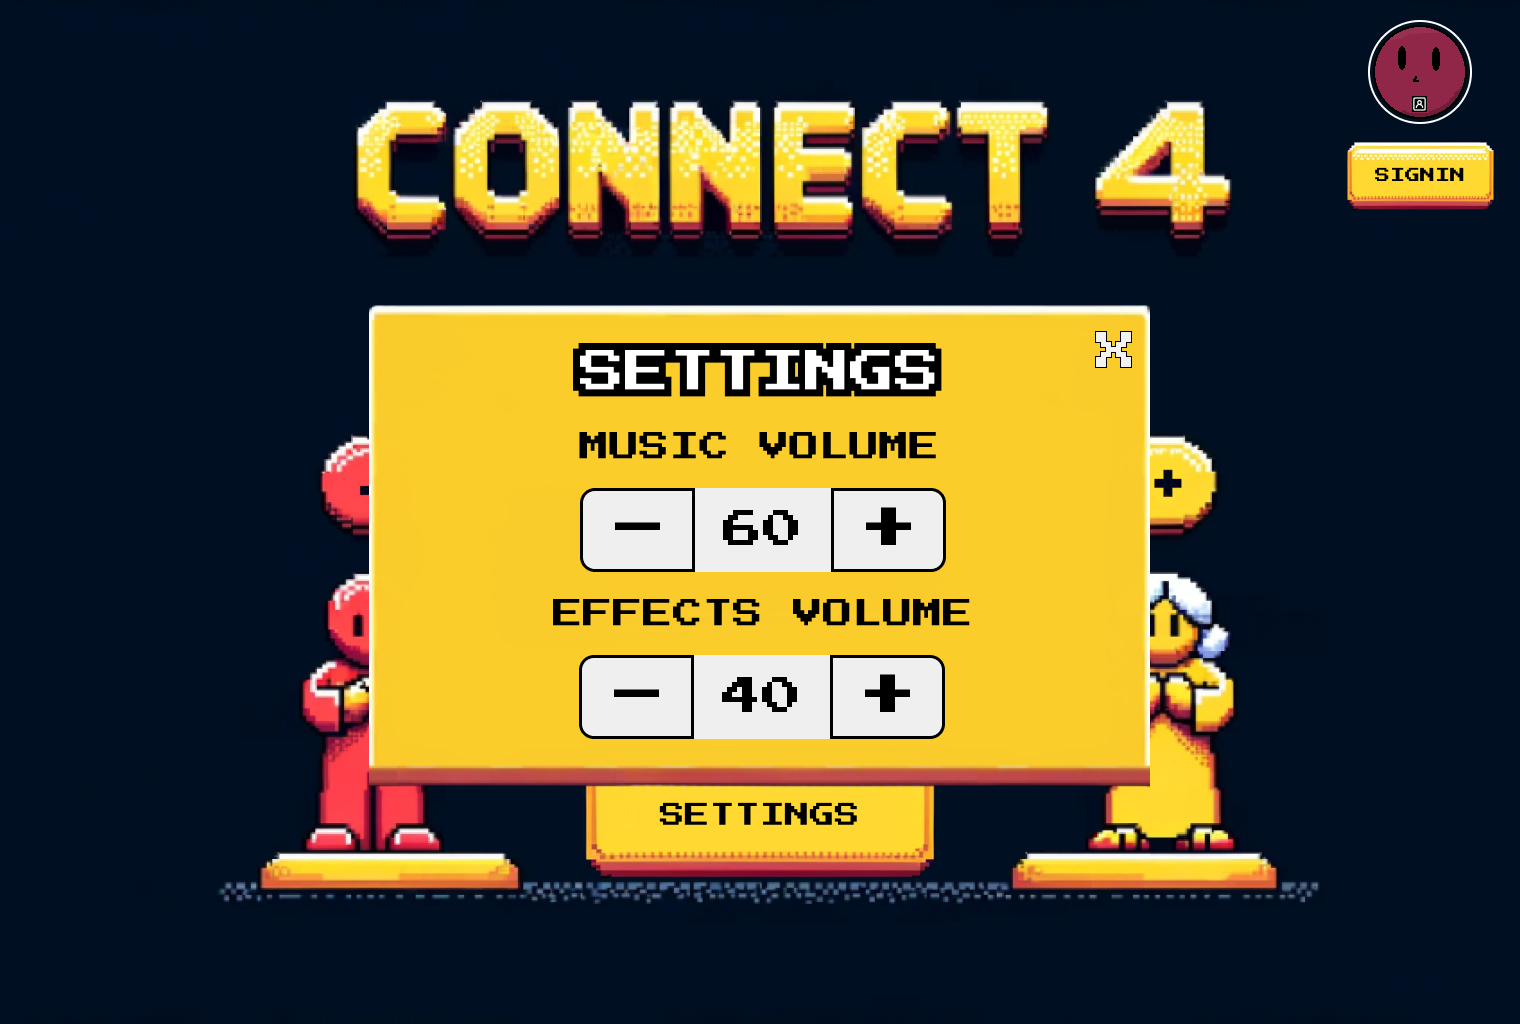
\includegraphics[width=0.8\textwidth]{Settings.png}
  \caption{Vyskakovacie okno s nastaveniami}
  \label{fig:settings}
\end{figure}

\subsection*{Obchod 1}
\begin{figure}[H]
  \centering
  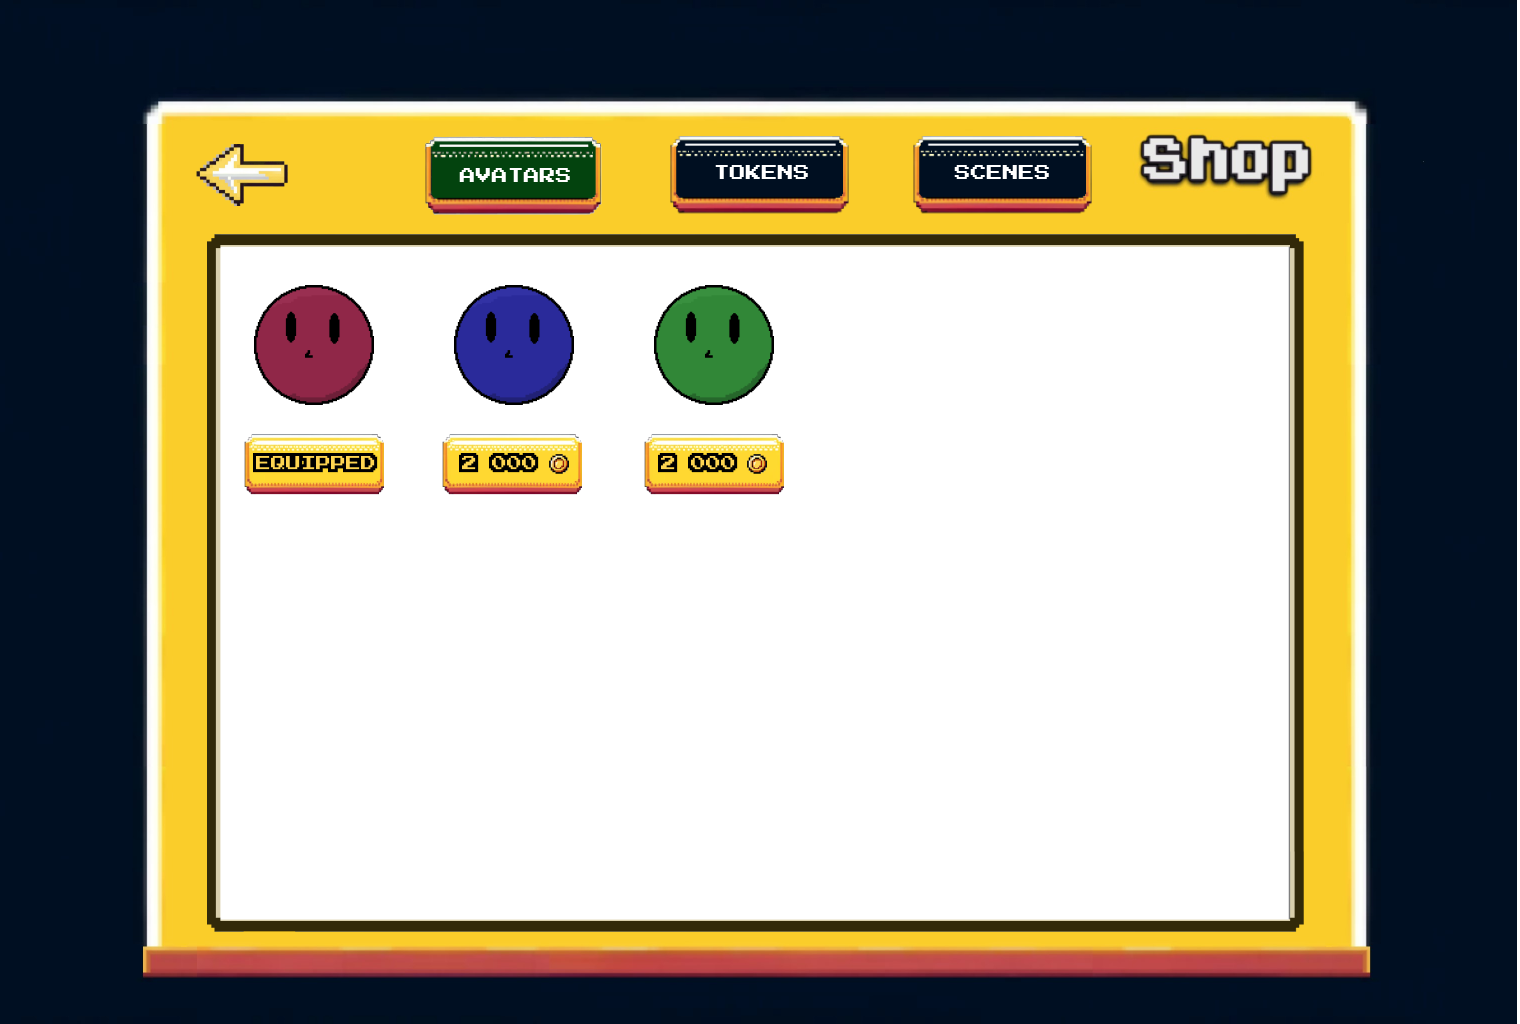
\includegraphics[width=0.8\textwidth]{ShopAvatars.png}
  \caption{Stránka obchodu s dostupnými avatarmi}
  \label{fig:shopAvatars}
\end{figure}

\subsection*{Obchod 2}
\begin{figure}[H]
  \centering
  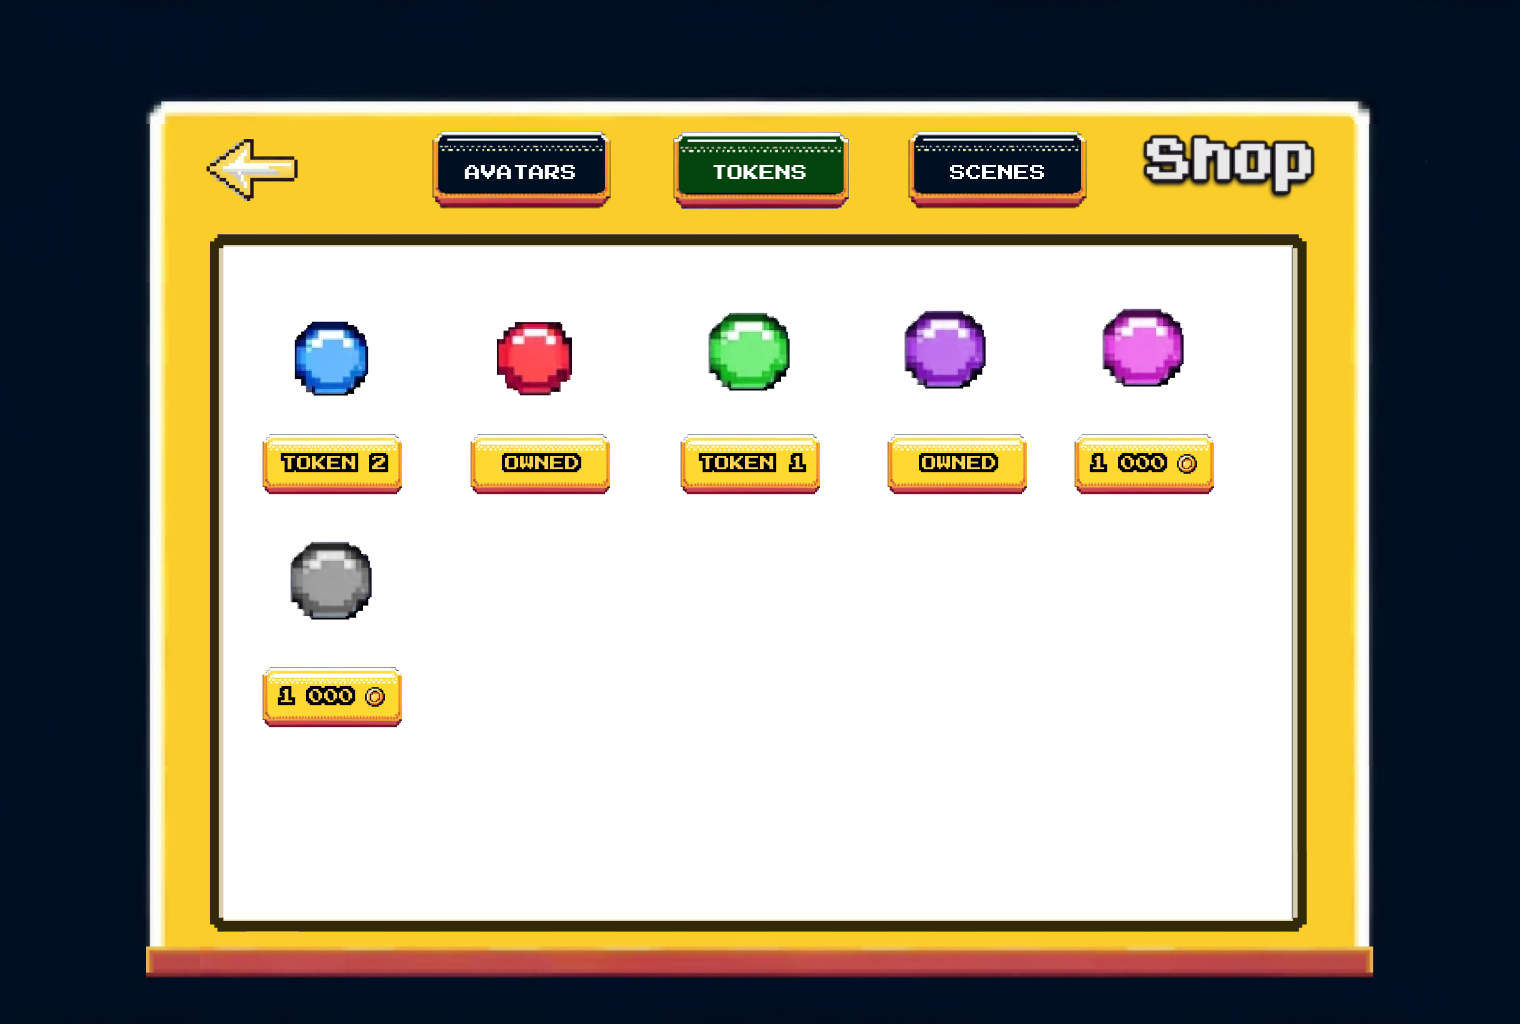
\includegraphics[width=0.8\textwidth]{ShopTokens.png}
  \caption{Stránka obchodu s dostupnými žetónmi}
  \label{fig:shopTokens}
\end{figure}

\subsection*{Obchod 3}
\begin{figure}[H]
  \centering
  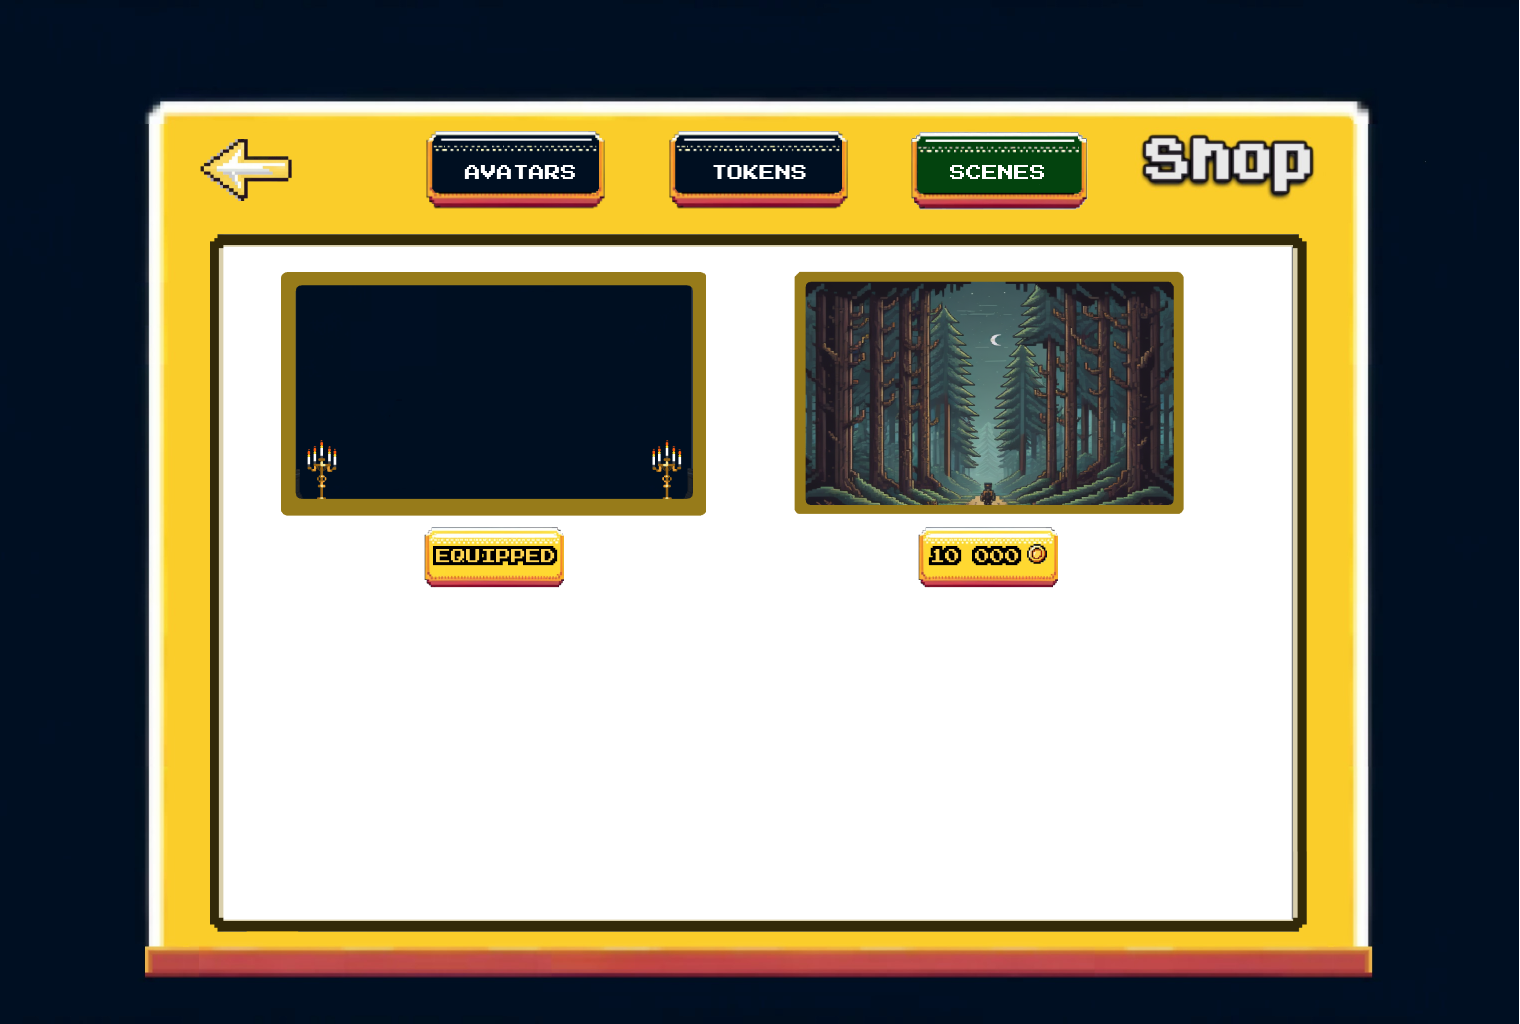
\includegraphics[width=0.8\textwidth]{ShopBack.png}
  \caption{Stránka obchodu s dostupnými pozadiami}
  \label{fig:shopBack}
\end{figure}

\subsection*{Riešenie potrieb užívateľov}
\begin{itemize}
  \item \textbf{Modifikovateľnosť:} Pokiaľ sa užívateľ prihlási, má možnosť zmeny 
               použitej scenérie na pozadí hry, avataru profilu a tokenu použitého pri hre.
  \item \textbf{Varianty:} Pridali sme variantu hry, ktorá má za úlohu udržať hru čo najdlhšie
                zaujímavú. Ide o variantu kde pri páde tokenu do hernej plochy, sa token
                ešte môže poodrážať a dopadnúť na iné políčko ako bolo pôvodne zamýšlané.
  \item \textbf{Vizuálny aspekt:} Rozhodli sme sa využiť pixel art ako zvolenú umeleckú formu.
                Zámienkou je vytvoriť atraktívnu hru pre nových užívateľov ako aj pre stálich hráčov.
\end{itemize}

\subsection*{Testovanie makety}
Na testovanie makety navrhnutej aplikácie boli oslovení rovankí respondenti ako pri vypĺňaní dotazníkov. Testovanie priebiehalo
počas osobného stretnutia. Respondentom bola pri teste predložené úlohy, ktoré mali bez akéhokoľvek postupu alebo pomoci splňiť.
Testované úlohy:
\begin{itemize}
  \item Kúpiť novú variantu tokenu
  \item Nastaviť kúpenú variantu tokenu pre druhého hráča
  \item Zmeniť si heslo
  \item Zmeniť hlasitosť 
  \item Zistiť počet odohratých zápasov
\end{itemize}
\subsection*{Testovacie metriky}
\begin{itemize}
    \item \textbf{Úspešnosť dokončených úloh:} Koľko úloh bolo dokončených úspešne (počet úspešných / celkový počet úloh)
    \item \textbf{Úspešnosť obnovy z chýb (Error Recovery Rate):} Koľko krát užívateľ po chybnom kliknutí úspešne dokončil úlohu (počet úspešných dokončení po chybe / počet chýb)
    \item \textbf{Čas strávený pri úlohe:} Ako dlho trvalo užívateľovi dokončiť úlohu?
\end{itemize}
\subsection*{Vyhodnotenie}
\begin{itemize}
    \item \textbf{Úspešnosť dokončených úloh:} 80\% (12 / 15 )
    \item \textbf{Úspešnosť obnovy z chýb:} 50\% ( 3 / 6 )
    \item \textbf{Čas strávený pri úlohe:} priemerne 25 sekúnd 
\end{itemize}
Testovaním bolo odhalených niekoľko nedostatkov, napríklad respondentom sa nebolo jasné že pokiaľ nie sú prihlásení, tak 
obchod nie je dostupný. Tento problém bude vyriešený pridaním vyskakovacieho okna, ktoré bude oznamovať že na prístup do obchodu je nutné sa prihlásiť. 
Ďaľší respondent poukázal na to že v obchode nie je jasné, ktoré varianty je schopný si kúpiť, pretože v obchode nevidí koľko hernej meny aktuálne má.
Riešením bude pridanie stavu meny do obchodu.

\section{Návrh riešienia aplikácie}
Po zvážení schopností a silných stránok tímu, sme ako programovací jazyk vybrali C\# .Ako platformu pre vývoj aplikácie WPF (Windows Presentation Foundation).
Na ukladanie dát je použitý relačný databázový systém SQLite. Aplikácia je postavená na modeli MVVM (Model\,-\,view\,-\,viewmodel).
\end{document}